\documentclass[12pt,a4paper,oneside]{report}

% -------------------------------------------------------------------
% B.E. Project Work-I report template for PVG's COET&M, Pune
% Editable LaTeX source. Diagrams are drawn in TikZ for portability.
% -------------------------------------------------------------------
\usepackage[a4paper,top=23.4mm,bottom=32mm,left=37mm,right=23.4mm]{geometry}
\usepackage[T1]{fontenc}
\usepackage[utf8]{inputenc}
\usepackage{newtxtext,newtxmath}
\usepackage{microtype}
\usepackage{setspace}
\usepackage{ragged2e}
\usepackage{graphicx}
\usepackage{array,booktabs,longtable,tabularx,multirow}
\usepackage{enumitem}
\usepackage{amsmath}
\usepackage{float}
\usepackage{etoolbox}
\usepackage{caption}
\usepackage{titlesec}
\usepackage{fancyhdr}
\usepackage{tikz}
\usetikzlibrary{arrows.meta,positioning,shapes.geometric,shapes.multipart,fit,calc,backgrounds,patterns}
\usepackage[hidelinks]{hyperref}
\usepackage{bookmark}
\usepackage{url}
\usepackage{array}
\usepackage{pdflscape}
\usepackage{rotating}
\usepackage{listings}

\setstretch{1.5}
\AtBeginEnvironment{tikzpicture}{\setstretch{1.0}\selectfont\setlength{\parskip}{0pt}}\tikzset{every node/.append style={execute at begin node=\setstretch{1.0}\selectfont}}
\setlength{\parindent}{1.25cm}
\setlength{\parskip}{0.45\baselineskip}
\setlength{\emergencystretch}{3em}
\setcounter{secnumdepth}{3}
\setcounter{tocdepth}{3}
\renewcommand{\arraystretch}{1.2}
\captionsetup{font=normalsize,labelfont=bf,justification=centering}
\captionsetup[table]{position=bottom,skip=6pt}
\captionsetup[figure]{position=bottom,skip=6pt}

\titleformat{\chapter}[display]
  {\centering\bfseries\fontsize{14}{17}\selectfont}
  {CHAPTER \thechapter}{0.6em}{\MakeUppercase}
\titlespacing*{\chapter}{0pt}{0pt}{1.2em}
\titleformat{\section}{\bfseries\fontsize{12}{14}\selectfont}{\thesection}{0.8em}{\MakeUppercase}
\titlespacing*{\section}{0pt}{1.2em}{0.6em}
\titleformat{\subsection}{\bfseries\fontsize{12}{14}\selectfont}{\thesubsection}{0.8em}{}
\titlespacing*{\subsection}{0pt}{0.8em}{0.35em}
\titleformat{\subsubsection}{\bfseries\itshape\fontsize{12}{14}\selectfont}{\thesubsubsection}{0.8em}{}
\titlespacing*{\subsubsection}{0pt}{0.65em}{0.25em}

\pagestyle{fancy}
\fancyhf{}
\renewcommand{\headrulewidth}{0pt}
\renewcommand{\footrulewidth}{0pt}
\fancyfoot[C]{\fontsize{10}{11}\selectfont Department of AI \& DS, PVGCOET\&M 2026-27\\[-1pt]\thepage}
\fancypagestyle{plain}{%
  \fancyhf{}
  \fancyfoot[C]{\fontsize{10}{11}\selectfont Department of AI \& DS, PVGCOET\&M 2026-27\\[-1pt]\thepage}
  \renewcommand{\headrulewidth}{0pt}}

\newcommand{\reporttitle}{AI-BASED MEDICAL REPRESENTATIVE VISIT PRIORITIZATION AND ROUTE OPTIMIZATION SYSTEM}
\newcommand{\college}{PVG's College of Engineering, Technology \& Management, Pune}
\newcommand{\department}{Department of Artificial Intelligence \& Data Science}
\newcommand{\guidename}{Prof. M. U. Buchade}
\newcommand{\studentone}{Bhakti Jayantilal Gundecha}
\newcommand{\studenttwo}{Parth Lokhande}
\newcommand{\studentthree}{Udaykiran Bitla}
\newcommand{\exone}{3071}
\newcommand{\extwo}{1020}
\newcommand{\exthree}{3056}

\tikzset{
  block/.style={draw,rectangle,rounded corners=2pt,align=center,minimum height=8mm,text width=33mm,inner sep=4pt},
  smallblock/.style={draw,rectangle,rounded corners=2pt,align=center,minimum height=7mm,text width=25mm,inner sep=3pt},
  decision/.style={draw,diamond,aspect=2,align=center,inner sep=1pt,text width=21mm},
  entity/.style={draw,rectangle,align=left,font=\footnotesize,text width=34mm,inner sep=4pt},
  umlclass/.style={draw,rectangle,align=left,text width=37mm,inner sep=4pt},
  line/.style={-Latex,thick},
  relation/.style={-Latex,thick},
  lifeline/.style={dashed,thick},
  plainnode/.style={draw,rectangle,align=center,inner sep=4pt}
}

\begin{document}

% ----------------------- FRONT MATTER -------------------------------
\begin{titlepage}
\thispagestyle{empty}
\setstretch{1.0}\setlength{\parskip}{0pt}
\begin{center}
\vspace*{8mm}
{\bfseries\fontsize{12}{15}\selectfont A PRELIMINARY REPORT ON}\par
\vspace{8mm}
{\bfseries\fontsize{16}{20}\selectfont \reporttitle}\par
\vspace{9mm}
{\fontsize{12}{15}\selectfont SUBMITTED TO THE SAVITRIBAI PHULE PUNE UNIVERSITY, PUNE\\
IN PARTIAL FULFILLMENT OF THE REQUIREMENTS FOR THE AWARD OF THE DEGREE OF}\par
\vspace{5mm}
{\bfseries\fontsize{14}{17}\selectfont BACHELOR OF ENGINEERING\\(ARTIFICIAL INTELLIGENCE \& DATA SCIENCE)}\par
\vspace{8mm}
{\fontsize{12}{15}\selectfont SUBMITTED BY}\par
\vspace{4mm}
\begin{tabular}{>{\raggedright\arraybackslash}p{92mm}r}
\textbf{\studentone} & \textbf{Exam No.: \exone}\\[3pt]
\textbf{\studenttwo} & \textbf{Exam No.: \extwo}\\[3pt]
\textbf{\studentthree} & \textbf{Exam No.: \exthree}\\
\end{tabular}\par
\vspace{8mm}
{\fontsize{12}{15}\selectfont Under the guidance of}\par
\vspace{2mm}
{\bfseries\fontsize{12}{15}\selectfont \guidename}\par
\vfill
{\bfseries\fontsize{14}{17}\selectfont DEPARTMENT OF ARTIFICIAL INTELLIGENCE \& DATA SCIENCE}\par
\vspace{3mm}
{\bfseries\fontsize{12}{15}\selectfont PUNE VIDYARTHI GRIHA'S COLLEGE OF ENGINEERING, TECHNOLOGY \& MANAGEMENT}\par
{\bfseries\fontsize{12}{15}\selectfont 44, VIDYANAGARI, PARVATI, PUNE 411009}\par
\vspace{4mm}
{\bfseries\fontsize{12}{15}\selectfont ACADEMIC YEAR 2026--2027}\par
\end{center}
\end{titlepage}

\clearpage
\pagenumbering{roman}
\thispagestyle{plain}
\begingroup\setstretch{1.0}\selectfont\setlength{\parskip}{0pt}
\begin{center}
{\bfseries\fontsize{12}{15}\selectfont SAVITRIBAI PHULE PUNE UNIVERSITY}\par
\vspace{2mm}
{\bfseries\fontsize{14}{17}\selectfont PVG'S COLLEGE OF ENGINEERING, TECHNOLOGY \& MANAGEMENT, PUNE}\par
\vspace{2mm}
{\bfseries\fontsize{12}{15}\selectfont \department}\par
\vspace{8mm}
{\bfseries\fontsize{14}{17}\selectfont CERTIFICATE}\par
\end{center}
\vspace{5mm}
\noindent This is to certify that the preliminary project report entitled \textbf{``\reporttitle''}, submitted by \textbf{\studentone} (Exam No. \exone), \textbf{\studenttwo} (Exam No. \extwo), and \textbf{\studentthree} (Exam No. \exthree), is a record of the work proposed and documented by them under the guidance of \textbf{\guidename}. The report is submitted in partial fulfilment of the requirements of Savitribai Phule Pune University for the award of the degree of Bachelor of Engineering in Artificial Intelligence and Data Science.

\vspace{14mm}
\noindent\begin{minipage}[t]{0.45\textwidth}
\centering
\rule{55mm}{0.4pt}\\
\guidename\\
Internal Guide\\
Department of AI \& DS
\end{minipage}
\hfill
\begin{minipage}[t]{0.45\textwidth}
\centering
\rule{55mm}{0.4pt}\\
Dr. Mrs. M. P. Atre\\
Head of Department\\
Department of AI \& DS
\end{minipage}
\vspace{12mm}
\begin{center}
\rule{65mm}{0.4pt}\\
Dr. S. R. Patil\\
I/C Principal\\
\college
\end{center}
\vfill
\noindent Place: Pune\hfill Date: \rule{35mm}{0.4pt}
\endgroup

\clearpage
\chapter*{ACKNOWLEDGEMENT}
\addcontentsline{toc}{chapter}{ACKNOWLEDGEMENT}
We would like to express our sincere gratitude to our internal guide, \guidename, for the guidance and feedback provided during the preparation of this preliminary project report. The discussions and review suggestions helped us define the project scope, separate prediction from route optimization, and document the design in a structured manner.

We are thankful to Dr. Mrs. M. P. Atre, Head of the Department of Artificial Intelligence and Data Science, and the faculty members of \college for their academic support and for providing the opportunity to undertake this project as part of the B.E. programme.

We also acknowledge the authors and maintainers of the research papers, technical documentation, libraries, and optimization tools referenced in this report. Their published work provides the theoretical and practical foundation for machine learning, vehicle routing with time windows, and web-based decision-support systems.

\vspace{10mm}
\begin{flushright}
\studentone\\
\studenttwo\\
\studentthree\\
(B.E. Artificial Intelligence \& Data Science)
\end{flushright}

\begingroup\setstretch{1.0}\selectfont\setlength{\parskip}{0.35\baselineskip}
\chapter*{ABSTRACT}
\addcontentsline{toc}{chapter}{ABSTRACT}
Medical Representatives (MRs) must visit several doctors within a limited working day. Each planned visit can differ in priority, appointment availability, duration, geographical location, previous visit outcome, and follow-up requirement. Manual planning and spreadsheet-based schedules can therefore lead to avoidable travel, waiting time, missed appointments, and limited visibility for managers. This report presents the design of an AI-based web application that integrates visit-priority prediction with constraint-based route optimization in one decision-support workflow.

The proposed system collects doctor master data, MR profiles, appointment records, historical visits, visit outcomes, and location information. After validation and preprocessing, a supervised machine-learning pipeline is intended to estimate the priority of each planned visit. A Random Forest classifier is proposed as the baseline model, with the final classification or ranking formulation to be confirmed after inspecting the quantity, consistency, and reliability of the available labels. The predicted priority is not used to generate a route by itself. Instead, it becomes one input to a routing engine that considers appointment time windows, service duration, MR working hours, start and end locations, and travel-time estimates. Google OR-Tools is proposed for solving a Vehicle Routing Problem with Time Windows (VRPTW). The result is a daily visit sequence with estimated timing and travel information.

The application is planned with React.js for the user interface, FastAPI and Python for backend services, scikit-learn for machine learning, Google OR-Tools for routing, and MySQL for persistence. Role-based interfaces are designed for MRs and managers. The report documents the problem definition, related work, software requirements, architecture, data model, UML diagrams, project plan, risks, security considerations, and evaluation methodology. Since implementation and experiments are still in progress, numerical claims of model accuracy or route improvement are not made. Evaluation will compare the proposed approach against a manual or simple baseline using prediction metrics and route-quality measures.

\noindent\textbf{Keywords:} Medical Representative, Visit Prioritization, Machine Learning, Random Forest, Route Optimization, VRPTW, Google OR-Tools, Decision Support System.
\endgroup

\tableofcontents
\listoffigures
\listoftables

\chapter*{LIST OF ABBREVIATIONS}
\addcontentsline{toc}{chapter}{LIST OF ABBREVIATIONS}
\begin{longtable}{>{\bfseries}p{28mm}p{100mm}}
AI & Artificial Intelligence\\
API & Application Programming Interface\\
CRUD & Create, Read, Update, Delete\\
DBMS & Database Management System\\
ER & Entity--Relationship\\
F1 & Harmonic mean of precision and recall\\
HTTP & Hypertext Transfer Protocol\\
ML & Machine Learning\\
MR & Medical Representative\\
ORM & Object-Relational Mapping\\
REST & Representational State Transfer\\
ROC-AUC & Receiver Operating Characteristic Area Under the Curve\\
SRS & Software Requirements Specification\\
UI & User Interface\\
UML & Unified Modeling Language\\
VRP & Vehicle Routing Problem\\
VRPTW & Vehicle Routing Problem with Time Windows\\
\end{longtable}

\chapter*{NOMENCLATURE}
\addcontentsline{toc}{chapter}{NOMENCLATURE}
\begin{longtable}{p{28mm}p{100mm}}
$D$ & Set of doctors or visit locations planned for a day.\\
$V$ & Set of routing nodes, including start/end locations.\\
$A$ & Set of feasible directed arcs between routing nodes.\\
$t_{ij}$ & Estimated travel time from node $i$ to node $j$.\\
$d_{ij}$ & Estimated distance from node $i$ to node $j$.\\
$s_i$ & Service duration for the visit at node $i$.\\
$[a_i,b_i]$ & Permitted appointment time window for visit $i$.\\
$H$ & MR working-hour horizon for the planned day.\\
$x_{ij}$ & Binary decision variable equal to 1 if the route travels directly from $i$ to $j$.\\
$p_i$ & Predicted priority score or class for visit $i$.\\
$u_i$ & Penalty associated with leaving important visit $i$ unserved.\\
$w_t,w_w,w_u$ & Weights for travel time, waiting time, and unserved-visit penalties.\\
\end{longtable}

% ----------------------- MAIN REPORT --------------------------------
\clearpage
\pagenumbering{arabic}
\chapter{INTRODUCTION}

\section{Project Idea}
The project proposes a web-based decision-support system that estimates the importance of planned doctor visits from historical and operational records, then generates a feasible daily visit route subject to appointment and working-hour constraints. It combines predictive modelling with operations research rather than treating doctor selection, scheduling, and navigation as unrelated activities.

\section{Motivation of the Project}
Medical Representatives perform field work that involves visiting doctors, communicating approved product information, recording visit outcomes, and arranging follow-ups. Their time is limited, and doctors are not available at identical hours or locations. A plan based only on manual judgement may ignore differences in follow-up urgency or generate unnecessary movement between geographically distant locations. A single system that shows why a visit is important and when it can feasibly be performed can support more consistent planning and more transparent monitoring. The intended application is a planning aid: the MR and manager remain responsible for reviewing the schedule and handling business exceptions.

\section{Background and Context}
The project joins two decision problems. Visit prioritization estimates the relative importance of a planned interaction. Route optimization determines a sequence and schedule that respects temporal and operational constraints. These problems are related but are not interchangeable. A high-priority doctor cannot automatically be visited first if the doctor is unavailable until later, and a short route is not necessarily a good route if it systematically omits important follow-ups.

The proposed workflow uses operational data as input, generates a priority output from a machine-learning model, and supplies that output to a constrained optimizer. The web application exposes the schedule and supporting information to an MR and provides aggregated activity information to a manager. This design is consistent with the separation of travel-cost modeling and time-window constraints demonstrated in established VRPTW literature and the OR-Tools routing examples \cite{solomon1987,ortoolsVRPTW}.

\begin{figure}[htbp]
\centering
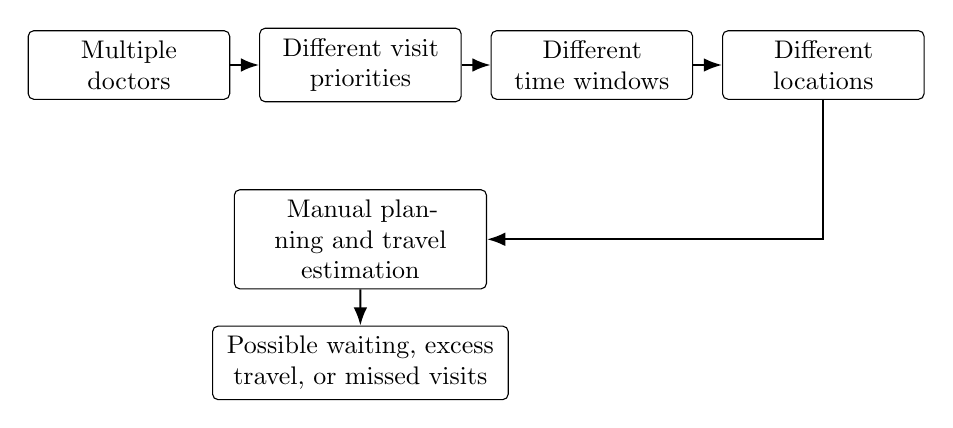
\begin{tikzpicture}[node distance=5mm and 4mm,scale=0.92,transform shape]
\node[block,text width=25mm] (doctors) {Multiple doctors};
\node[block,right=of doctors,text width=25mm] (priority) {Different visit priorities};
\node[block,right=of priority,text width=25mm] (windows) {Different time windows};
\node[block,right=of windows,text width=25mm] (locations) {Different locations};
\node[block,below=12mm of priority,text width=32mm] (manual) {Manual planning and travel estimation};
\node[block,below=of manual,text width=38mm] (outcome) {Possible waiting, excess travel, or missed visits};
\draw[line] (doctors)--(priority);
\draw[line] (priority)--(windows);
\draw[line] (windows)--(locations);
\draw[line] (locations.south) |- (manual.east);
\draw[line] (manual)--(outcome);
\end{tikzpicture}
\caption{Problem context for daily MR visit planning.}
\label{fig:problem-context}
\end{figure}

\section{Problem Idea and Existing Practice}
A typical manual process begins with a list of doctors assigned to a territory. The MR or manager checks appointments, chooses visits, estimates travel, and prepares a daily schedule. Maps may help navigate between two points but do not, by themselves, resolve visit selection, visit duration, appointment windows, and the complete daily route as one optimization problem. Separate appointment records and static schedules also make it difficult to re-plan when an appointment changes.

\begin{table}[htbp]
\centering
\begin{tabularx}{\textwidth}{p{40mm}X}
\toprule
\textbf{Existing practice} & \textbf{Limitation addressed by the project}\\
\midrule
Manual prioritization & Can vary by individual judgement and may not consistently use historical follow-up evidence.\\
Spreadsheet planning & Becomes difficult to maintain as doctor records, appointment changes, and territories grow.\\
Map navigation & Optimizes navigation between points, not the full appointment-constrained schedule.\\
Separate appointment records & Does not necessarily coordinate priority, service duration, and every stop in the route.\\
Static daily plan & Requires manual changes when appointments or visit outcomes change.\\
Limited analytics & Makes it harder for managers to compare planned, completed, pending, and high-priority visits.\\
\bottomrule
\end{tabularx}
\caption{Existing approach and identified limitations.}
\label{tab:existing-limitations}
\end{table}

\section{Motivation for Integrating Prediction and Optimization}
The project is not intended to replace field judgement with a fully autonomous decision. Instead, it provides structured information to help a user decide which visits are important and how they can be scheduled. Machine learning can estimate priority when reliable historical labels exist. A routing optimizer can then use the output alongside explicit constraints. The separation also makes the system easier to audit: a priority prediction can be inspected independently from a route decision.

\section{Organization of the Report}
Chapter 1 introduces the problem and motivation. Chapter 2 reviews related work. Chapter 3 defines the problem, scope, outcomes, and constraints. Chapter 4 presents the project plan and risk management. Chapter 5 specifies functional and non-functional requirements. Chapter 6 documents system, data, and UML design. Chapter 7 summarizes advantages, limitations, and applications. Chapter 8 concludes the report and identifies the next stage of implementation. References and annexures follow the main chapters.

\chapter{LITERATURE SURVEY}

\section{Introduction}
Research relevant to this project falls into several overlapping areas: vehicle routing, routing with appointment windows, sales-force and physician-detailing planning, dynamic routing, supervised classification, and software-based decision support. Classical routing work explains why large route spaces need systematic algorithms, while later VRPTW research adds explicit visit windows and improved heuristics. Predictive modelling supplies an estimate of visit importance, but it does not solve the route sequencing problem by itself.

\section{Review of Related Work}
\subsection{Classical Vehicle Routing}
Dantzig and Ramser formalized an early truck-dispatching problem and demonstrated the importance of computational methods for routing multiple service points from a depot \cite{dantzig1959}. Clarke and Wright proposed a savings-based method that constructs economical routes by combining deliveries that would otherwise be served separately \cite{clarke1964}. These studies established the principle that route planning can be framed as a combinatorial optimization problem rather than handled only by visual inspection.

Laporte reviewed exact and approximate algorithms for the vehicle routing problem and organized the main families of solution methods \cite{laporte1992}. Toth and Vigo later consolidated models, algorithms, and variants in a comprehensive treatment of vehicle routing \cite{tothvigo2014}. This project inherits the routing formulation but adds the particular requirements of a field representative whose visits have time windows, heterogeneous importance, and recorded follow-up outcomes.

\subsection{Vehicle Routing with Time Windows}
Solomon studied route construction and scheduling when customer visits must be made within specified time windows. The paper introduced benchmark instances and compared algorithms under different window characteristics \cite{solomon1987}. Solomon and Desrosiers surveyed routing and scheduling problems constrained by time windows, emphasizing that temporal constraints affect both feasibility and algorithm design \cite{solomonDesrosiers1988}.

Br\"aysy and Gendreau reviewed construction and local-search algorithms for the VRPTW and discussed how heuristic methods should be compared \cite{braysy2005a}. Their follow-up survey covers metaheuristic methods for the same class of problem \cite{braysy2005b}. Pisinger and Ropke introduced a general heuristic framework capable of addressing several vehicle-routing variants \cite{pisinger2007}. These works motivate a baseline-versus-proposed evaluation rather than assuming that a solver improves every route without empirical comparison.

The Google OR-Tools documentation provides a practical formulation of the VRPTW using a time matrix, time-window ranges, vehicle starts and ends, and a routing search strategy \cite{ortoolsVRPTW}. The project uses this as implementation guidance. OR-Tools requires travel costs and time data; it does not create geographically accurate travel times automatically. The source of the distance-time matrix must therefore be declared and evaluated separately.

\subsection{Dynamic and Time-Dependent Routing}
Pillac and colleagues reviewed dynamic vehicle-routing problems, distinguishing information available before planning from information arriving during execution \cite{pillac2013}. The key implication for an MR workflow is that appointment changes and field events may invalidate a route, so a later iteration should support controlled route regeneration. Bektas and Laporte's work on the pollution-routing problem illustrates how routing objectives can extend beyond distance to operational consequences such as fuel use and emissions \cite{bektas2011}. For this academic prototype, the primary focus remains travel time, waiting, visit coverage, and feasibility; environmental measures can be added where reliable data is available.

\subsection{Physician Detailing and Sales Representative Planning}
Yi, Anandalingam, and Sorrell developed an expert-system approach to physician-detailing planning that combines knowledge about physician response with neural-network modelling and nonlinear programming \cite{yi2003}. Yi and colleagues later examined a knowledge-based method for planning the sequence of product detailing, with a hybrid of neural networks and nonlinear optimization \cite{yi2010}. These works are particularly relevant because they treat physician interactions as resource-allocation decisions and demonstrate the value of integrating domain information with optimization.

The Review III presentation also identifies related studies by Zhang and colleagues on pharmaceutical sales-representative routing, Rhee and Yi on physician-interest prediction, Bouatouche and Belkadi on sales-representative planning, and Shala and colleagues on field-service planning. The supplied slide deck does not include full paper titles, venues, years, or DOIs for these entries. They are therefore treated here as areas identified during the project review, not as fully verified bibliographic records. Their references should be completed by the project team before final submission.

\subsection{Machine Learning and Random Forests}
Breiman introduced Random Forests as an ensemble of tree predictors trained with randomized samples and feature selection \cite{breiman2001}. The method is a reasonable baseline for tabular operational data because it can model non-linear relationships and interactions without requiring all features to be transformed into a linear scale. It can also estimate class probabilities, which can be useful if the optimizer needs a graded priority score rather than only a text label.

Pedregosa and colleagues described scikit-learn as a consistent Python machine-learning toolkit with estimators and evaluation tools for common learning tasks \cite{pedregosa2011}. The project proposes a preprocessing pipeline, train/test separation, and a Random Forest baseline. The choice must be revisited if the training data lacks dependable priority labels, is too small, or contains highly imbalanced classes. Under those conditions, a transparent rule-based ranking may be a more defensible initial approach than training a model whose output cannot be validated.

\subsection{Evaluation Methods}
Fawcett explained Receiver Operating Characteristic analysis and its use in evaluating binary classifiers across decision thresholds \cite{fawcett2006}. Davis and Goadrich discussed the relationship between precision-recall and ROC curves \cite{davis2006}; Saito and Rehmsmeier argued that precision-recall plots are particularly informative in imbalanced classification settings \cite{saito2015}. Accordingly, this report proposes accuracy, precision, recall, F1-score, confusion matrix, and ROC-AUC where appropriate. Metrics will be reported by class, and performance on high-priority visits will be inspected specifically instead of relying on accuracy alone.

\section{Summary of Surveyed Literature}
\begin{longtable}{>{\RaggedRight\arraybackslash}p{30mm}>{\RaggedRight\arraybackslash}p{33mm}>{\RaggedRight\arraybackslash}p{35mm}>{\RaggedRight\arraybackslash}p{34mm}}
\caption{Summary of relevant literature and its relationship to the project.}\label{tab:lit-survey}\\
\toprule
\textbf{Study} & \textbf{Main focus} & \shortstack[l]{\textbf{Method /}\\\textbf{Contribution}} & \shortstack[l]{\textbf{Relevance or}\\\textbf{limitation}}\\
\midrule
\endfirsthead
\toprule
\textbf{Study} & \textbf{Main focus} & \shortstack[l]{\textbf{Method /}\\\textbf{Contribution}} & \shortstack[l]{\textbf{Relevance or}\\\textbf{limitation}}\\
\midrule
\endhead
Dantzig and Ramser \cite{dantzig1959} & Truck dispatching & Early computational routing formulation & General routing foundation; not MR-specific.\\
Clarke and Wright \cite{clarke1964} & Multi-stop routing & Savings heuristic & Useful as a simple baseline; does not predict visit priority.\\
Solomon \cite{solomon1987} & VRPTW & Test instances and heuristics & Supports time-window modelling and comparative testing.\\
Solomon and Desrosiers \cite{solomonDesrosiers1988} & Time-window routing & Survey of routing/scheduling problems & Explains how temporal feasibility changes the problem.\\
Laporte \cite{laporte1992} & VRP algorithms & Review of exact and approximate methods & Establishes algorithm families and computational trade-offs.\\
Br\"aysy and Gendreau \cite{braysy2005a} & VRPTW heuristics & Construction and local search survey & Highlights baseline selection and algorithm comparison.\\
Br\"aysy and Gendreau \cite{braysy2005b} & VRPTW metaheuristics & Review of metaheuristic methods & Relevant to difficult constrained instances.\\
Pisinger and Ropke \cite{pisinger2007} & General VRP variants & Unified heuristic framework & Supports flexible routing formulations.\\
Pillac et al. \cite{pillac2013} & Dynamic VRP & Survey of dynamic problems & Motivates re-planning after changes.\\
Bektas and Laporte \cite{bektas2011} & Pollution routing & Routing with environmental cost & Suggests future objective extensions.\\
Yi et al. \cite{yi2003} & Physician detailing & Neural networks with nonlinear optimization & Domain-specific evidence for integrated planning.\\
Yi et al. \cite{yi2010} & Detailing-plan quality & Knowledge-based weights and hybrid modelling & Supports combining domain knowledge with prediction.\\
Breiman \cite{breiman2001} & \shortstack[l]{Classification/\\regression} & Random Forest ensemble & Proposed baseline for visit-priority prediction.\\
Pedregosa et al. \cite{pedregosa2011} & ML tooling & scikit-learn library & Practical pipeline and model evaluation support.\\
Fawcett \cite{fawcett2006} & Classifier evaluation & ROC analysis & Helps assess discrimination across thresholds.\\
Davis and Goadrich \cite{davis2006} & Classifier evaluation & Precision-recall and ROC relationship & Supports suitable metric selection.\\
Saito and Rehmsmeier \cite{saito2015} & Imbalanced learning & Precision-recall evaluation analysis & Relevant if priority classes are imbalanced.\\
Liu et al. \cite{liu2023} & VRPTW literature & Systematic review of recent methods & Shows modern VRPTW work uses complex methods and constraints.\\
Google OR-Tools \cite{ortoolsVRPTW} & Practical routing solver & Time dimension and time-window constraints & Direct reference for the proposed optimization module.\\
React documentation \cite{reactdocs} & Frontend UI & Component-based UI development & Supports dashboards and user interaction.\\
FastAPI documentation \cite{fastapidocs} & Backend APIs & Python API framework and validation & Supports service separation and request validation.\\
MySQL documentation \cite{mysqldocs} & Relational persistence & Database engine and SQL features & Supports structured operational data.\\
\bottomrule
\end{longtable}

\section{Research Gap}
The reviewed material covers physician targeting, sales-force planning, appointment scheduling, vehicle routing, and field-service optimization, but these themes are commonly formulated with different assumptions and objectives. The project-specific gap is the integration of a transparent visit-priority output with a route optimizer that explicitly checks appointment windows, service duration, MR working hours, and travel time in one MR-facing workflow.

The intended contribution is not a claim of a new routing algorithm. It is an applied system design that links a data-driven priority estimate to a constraint-based route and presents both to operational users. Its value must be demonstrated through evaluation on approved real or synthetic data.

\begin{figure}[htbp]
\centering
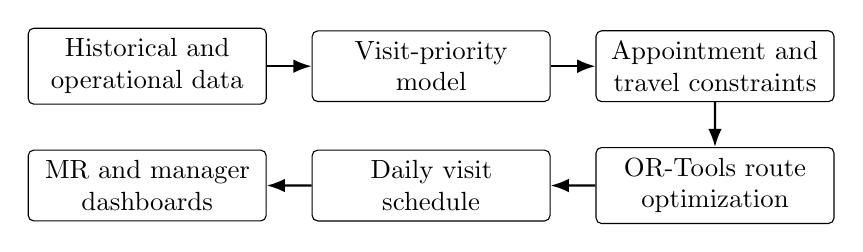
\begin{tikzpicture}[node distance=6mm,scale=0.95,transform shape]
\node[block,text width=29mm] (data) {Historical and operational data};
\node[block,right=of data,text width=29mm] (ml) {Visit-priority model};
\node[block,right=of ml,text width=29mm] (constraints) {Appointment and travel constraints};
\node[block,below=of constraints,text width=29mm] (opt) {OR-Tools route optimization};
\node[block,left=of opt,text width=29mm] (plan) {Daily visit schedule};
\node[block,left=of plan,text width=29mm] (dash) {MR and manager dashboards};
\draw[line] (data)--(ml);\draw[line] (ml)--(constraints);\draw[line] (constraints)--(opt);\draw[line] (opt)--(plan);\draw[line] (plan)--(dash);
\end{tikzpicture}
\caption{Research contribution: integration of priority prediction and feasible routing.}
\label{fig:research-gap}
\end{figure}

\chapter{PROBLEM DEFINITION AND SCOPE}

\section{Problem Statement}
Medical Representatives must visit multiple doctors during a workday, but each doctor may have a different importance level, availability window, location, service duration, and follow-up requirement. The representative must complete as many valuable visits as possible without violating appointment and working-hour constraints. Manual planning does not consistently integrate all of these factors, while generic map navigation only supports part of the task.

The problem is to design and implement a web-based decision-support system that (i) estimates the priority of planned visits from historical and operational data, (ii) finds a feasible and efficient visit sequence under temporal and travel constraints, and (iii) displays daily planning and activity information to MRs and managers. The quality of the final schedule depends on input quality, travel-time data, the available appointment windows, and the selected optimization objective.

\section{Goals and Objectives}
The overall goal is to support data-informed field planning while preserving the ability for users to inspect and override operational decisions. Specific objectives are:
\begin{enumerate}[leftmargin=1.2cm]
\item Define and validate data entities for doctors, MRs, visits, appointments, predicted priorities, routes, and route stops.
\item Prepare a repeatable data-cleaning and feature-engineering pipeline for historical and operational records.
\item Establish a baseline priority-prediction model, initially a Random Forest classifier if adequate labels are available.
\item Model working hours, doctor availability, visit duration, appointment windows, and travel times as routing constraints.
\item Use Google OR-Tools to produce a feasible route that balances travel effort and visit value.
\item Provide separate role-based views for MR day planning and manager-level monitoring.
\item Evaluate model quality and route quality against transparent baselines without presuming improvements before experiments.
\end{enumerate}

\section{Statement of Scope}
\subsection{Included in the Prototype}
The planned prototype includes user authentication and role-based access; doctor and MR master data; appointment and visit management; priority inference; route generation; daily schedule display; visit status updates; and manager dashboard summaries. It will support a limited experimental territory and a bounded daily set of visit candidates appropriate for testing. The optimizer will accept a travel-time matrix produced by a permitted map service, agency-approved data, precomputed routes, or a controlled simulation.

\subsection{Outside the Initial Scope}
The initial academic prototype does not require patient medical records, does not guarantee live traffic data, and does not claim integration with a commercial pharmaceutical CRM. Full GPS tracking, mobile application deployment, automated rescheduling with external calendars, and production-grade multi-city scaling are future extensions. Real-time performance and business benefits will not be asserted without experiments.

\subsection{Inputs and Outputs}
Major inputs include doctor ID, territory, location coordinates, availability window, typical visit duration, MR working start/end times, start/end locations, planned appointment date and time, previous visit history, visit outcome, follow-up flag, and priority labels where available. Inputs must be validated for missing IDs, invalid coordinates, impossible time windows, invalid durations, and inconsistent relationships.

The system is expected to output the predicted priority category or score, a proposed visit order, estimated arrival/start times, travel time and distance where available, unserved visits with reasons where detectable, and dashboard summaries of planned/completed/pending activity. The schedule is a recommendation subject to review by authorized users.

\section{Software Context}
The project is a web-based operational decision-support application. The React frontend communicates with a FastAPI backend through REST endpoints. The backend manages authentication, validation, domain logic, the priority-prediction pipeline, and route optimization. MySQL stores structured entities. scikit-learn provides the model implementation, and Google OR-Tools provides routing search and time-window constraints. Map or routing data is provided by an external service or controlled input dataset, depending on the experiment setup.

\section{Major Constraints}
\begin{enumerate}[leftmargin=1.2cm]
\item \textbf{Data quality:} Missing historical visits, incomplete labels, invalid coordinates, or inconsistent appointment records can reduce prediction and routing quality.
\item \textbf{Label availability:} Supervised learning requires priority labels with a consistent meaning. If the agency cannot supply them, the project must use an explicitly documented rule-based baseline or ranking formulation.
\item \textbf{Appointment feasibility:} High priority cannot override a hard appointment window unless a user explicitly changes the constraint.
\item \textbf{Routing complexity:} VRPTW is combinatorial; exact optimality cannot be guaranteed for every practical instance within a useful response time. The system should favour a feasible solution and transparently report infeasibility.
\item \textbf{Travel-time uncertainty:} A precomputed matrix may not reflect live traffic or temporary road conditions.
\item \textbf{Privacy:} Only data needed for scheduling should be stored; synthetic identifiers should be preferred for academic experiments.
\item \textbf{Prototype boundary:} The technology stack and available development time limit initial scale and integration scope.
\end{enumerate}

\section{Methodologies of Problem Solving and Efficiency Issues}
Three options are considered. Manual or spreadsheet planning has a low setup cost but depends heavily on user effort. A simple nearest-neighbour or fixed-priority ordering algorithm is fast and transparent but may create poor schedules under time windows. The proposed pipeline first predicts visit priority and then applies a constrained optimizer. The third option is more involved but allows objective comparison between data-informed priority and a feasible sequence.

Efficiency will be assessed using total travel time, total distance, waiting time, number of completed visits, unserved visits, time-window violations, and computation time. Prediction will be assessed independently using class-sensitive metrics. This separation helps determine whether a weak outcome originates in the ML layer, the travel-time input, or the optimization layer.

\section{Multi-Core, Embedded and Distributed Computing Context}
The prototype is a conventional client-server web application and does not require embedded computing. Distributed computing is present in the broad sense that browser-based clients communicate with a backend service and database over a network. The ML and optimization tasks may run on the backend. Multi-core execution can be used by underlying numerical libraries or server processes, but parallel computation is not a design requirement for the first version. If the system later serves multiple territories or MRs concurrently, task queues and isolated optimization jobs may help manage load.

\section{Expected Outcomes}
The expected outcome is a documented and testable prototype design with a validated data model, REST interface, priority-prediction pipeline, route-optimization module, MR dashboard, manager dashboard, and evaluation harness. A successful prototype should produce feasible routes for the supported test cases, display any unscheduled visits clearly, protect role-specific records, and provide reproducible baseline comparisons. Quantitative improvements will be reported only after running experiments.

\section{Applications}
Potential use cases include daily doctor-visit planning for pharmaceutical representatives, territory-based field sales scheduling, prioritization of follow-up visits, manager monitoring of daily field activities, and research on integrating prediction with route optimization. Similar techniques may also apply to non-medical field-service workflows, provided their business rules and privacy requirements are separately modelled.

\section{Hardware Resources Required}
\begin{table}[htbp]
\centering
\begin{tabularx}{\textwidth}{c p{35mm} p{35mm} X}
\toprule
\textbf{No.} & \textbf{Parameter} & \shortstack[l]{\textbf{Suggested}\\\textbf{minimum}} & \textbf{Justification}\\
\midrule
1 & CPU & Dual-core 2 GHz or better & Suitable for application development and small test datasets.\\
2 & RAM & 4 GB minimum; 8 GB recommended & Allows browser, editor, database, and backend services to run together.\\
3 & Storage & 5 GB free workspace & Source, sample datasets, environment files, and logs.\\
4 & Display & 1366 $\times$ 768 or better & Supports development and dashboard testing.\\
5 & Network & Stable internet access when external APIs are used & Needed for package installation and any external routing service.\\
\bottomrule
\end{tabularx}
\caption{Suggested development hardware requirements.}
\end{table}

\section{Software Resources Required}
\begin{table}[htbp]
\centering
\begin{tabularx}{\textwidth}{p{36mm}X}
\toprule
\textbf{Category} & \textbf{Proposed software or tool}\\
\midrule
Operating system & Windows, Linux, or macOS development environment.\\
Frontend & React.js and a modern browser.\\
Backend & Python with FastAPI.\\
Machine learning & pandas/NumPy for data handling and scikit-learn for preprocessing and Random Forest.\\
Optimization & Google OR-Tools routing library.\\
Database & MySQL relational database.\\
API testing & OpenAPI interface exposed by FastAPI and an HTTP client.\\
Version control & Git with a remote repository as available.\\
\shortstack[l]{Diagramming/\\documentation} & LaTeX/TikZ or an equivalent diagram tool.\\
\bottomrule
\end{tabularx}
\caption{Proposed software resources.}
\end{table}

\chapter{PROJECT PLAN}

\section{Project Estimates}
Project estimates are planning estimates for the academic prototype, not vendor quotations or approved expenditure. The team should update them after the chosen dataset, hosting approach, and any external API requirements are confirmed.

\subsection{Cost Estimate}
The design can be developed with open-source languages and libraries. The following plan assumes local development, a local or student-accessible MySQL instance, and public documentation. If a commercial map API, cloud hosting, SMS, or production authentication service is adopted, those costs must be recorded separately.
\begin{table}[htbp]
\centering
\begin{tabularx}{\textwidth}{p{42mm}p{40mm}X}
\toprule
\textbf{Resource} & \textbf{Cost approach} & \textbf{Note}\\
\midrule
Development tools & Open-source / existing access & No licence cost assumed in this estimate.\\
Database and backend & Local development & Hosting is a separate future decision.\\
Routing data & Approved/free data or controlled matrix for prototype & API terms, quotas, and billing must be checked before use.\\
Test dataset & Synthetic or approved anonymized data & No patient medical records are required by the core workflow.\\
Deployment & To be determined & No production hosting amount is asserted.\\
\bottomrule
\end{tabularx}
\caption{Preliminary cost-estimation basis.}
\end{table}

\subsection{Time Estimate}
The project can be managed in phases. The schedule below is a proposed sequence rather than a record of completed work. Actual dates should be filled from the team's sanctioned project planner.
\begin{table}[htbp]
\centering
\begin{tabularx}{\textwidth}{c p{43mm} c X}
\toprule
\textbf{No.} & \textbf{Task} & \textbf{Effort} & \textbf{Exit condition}\\
\midrule
1 & Problem definition and survey & 2 weeks & Scope and review references consolidated.\\
2 & Requirement analysis and data schema & 2 weeks & Approved SRS and entity relationships.\\
3 & UI design and backend skeleton & 2 weeks & Role flows and API contract agreed.\\
4 & Data preparation and ML baseline & 2--3 weeks & Reproducible preprocessing and baseline metrics.\\
5 & Route optimizer and travel matrix & 2--3 weeks & Feasible sample routes with test cases.\\
6 & Application integration & 2 weeks & End-to-end workflow available in development.\\
7 & Testing and evaluation & 2 weeks & Baseline comparison and defect log.\\
8 & Documentation and demonstration & 1--2 weeks & Report, slides, and demo checklist.\\
\bottomrule
\end{tabularx}
\caption{Proposed development estimate.}
\end{table}

\section{Project Resources}
Resources include three student team members, the internal guide, a development computer, internet access where required, Python and JavaScript environments, MySQL, Git, and the technical documentation for scikit-learn and OR-Tools. Responsibilities should be assigned explicitly, but each module should be reviewed by at least one other team member to reduce integration risk.

\subsection{Team Organization}
\begin{table}[htbp]
\centering
\begin{tabularx}{\textwidth}{p{48mm}p{43mm}X}
\toprule
\textbf{Team member} & \textbf{Exam No.} & \textbf{Shared responsibilities}\\
\midrule
\studentone & \exone & Requirements, data model, testing and report preparation; module ownership to be confirmed by the team.\\
\studenttwo & \extwo & System design, application integration, route workflow and documentation; module ownership to be confirmed by the team.\\
\studentthree & \exthree & ML pipeline, UI/backend implementation and validation; module ownership to be confirmed by the team.\\
\bottomrule
\end{tabularx}
\caption{Project team and initial coordination plan.}
\end{table}

\subsection{Management Reporting and Communication}
The team should maintain a single list of requirements, issue status, open data assumptions, test cases, and design decisions. Each review should report what was completed, what remains in progress, risks that need guidance, and evidence from tests. API contracts and database changes should be shared before integration rather than discovered only at the final demo. Decisions that affect the project scope should be confirmed with the internal guide.

\section{Risk Management with Respect to NP-Hard Analysis}
Vehicle routing with time windows is a combinatorial optimization problem. The number of possible sequences increases rapidly as the number of visit locations grows. A practical solver may use heuristics and search limits to find good feasible solutions. Consequently, project risk management must address computational time, feasible-solution detection, changing inputs, and the reliability of evaluation data.

\subsection{Risk Identification and Analysis}
\begin{longtable}{c >{\RaggedRight\arraybackslash}p{39mm} >{\RaggedRight\arraybackslash}p{20mm} >{\RaggedRight\arraybackslash}p{20mm} >{\RaggedRight\arraybackslash}p{35mm}}
\caption{Project risk analysis.}\label{tab:risk-analysis}\\
\toprule
\textbf{ID} & \textbf{Risk} & \textbf{Likelihood} & \textbf{Impact} & \textbf{Monitoring indicator}\\
\midrule
\endfirsthead
\toprule
\textbf{ID} & \textbf{Risk} & \textbf{Likelihood} & \textbf{Impact} & \textbf{Monitoring indicator}\\
\midrule
\endhead
R1 & Historical data unavailable or too small & Medium & High & Missing fields, low row count, unavailable labels.\\
R2 & Priority labels inconsistent across records & Medium & High & Disagreement between business definitions and stored categories.\\
R3 & Invalid or missing coordinates & Medium & High & Failed coordinate checks or impossible distance values.\\
R4 & Route infeasible due to tight windows & Medium & High & No feasible assignment for a test instance.\\
R5 & Optimization runtime too high & Medium & Medium & Solver exceeds configured time budget.\\
R6 & Appointment changes after route generation & High & Medium & Stale plan or repeated manual edits.\\
R7 & Travel-time matrix is inaccurate & Medium & High & Large difference between estimated and observed times.\\
R8 & Class imbalance affects high-priority recall & Medium & High & Few high-priority examples or low recall.\\
R9 & API or database failure & \shortstack[l]{Low/\\Medium} & High & Timeouts, failed writes, service unavailability.\\
R10 & Unauthorized access to operational data & \shortstack[l]{Low/\\Medium} & High & Failed role checks or access-control defects.\\
R11 & Integration mismatch among modules & Medium & Medium & Incompatible data formats or contract changes.\\
R12 & Scope expansion reduces testing time & Medium & Medium & Repeated new features close to review deadlines.\\
\bottomrule
\end{longtable}

\subsection{Risk Mitigation, Monitoring and Management}
\begin{longtable}{p{18mm}p{49mm}p{63mm}}
\caption{Risk mitigation plan.}\label{tab:risk-mitigation}\\
\toprule
\textbf{Risk ID} & \textbf{Mitigation} & \textbf{Response if observed}\\
\midrule
\endfirsthead
\toprule
\textbf{Risk ID} & \textbf{Mitigation} & \textbf{Response if observed}\\
\midrule
\endhead
R1--R2 & Define required fields and label meanings early; prefer approved anonymized or synthetic data for the prototype. & Record limitations; switch to a transparent ranking baseline if supervised labels are unreliable.\\
R3 & Validate latitude/longitude ranges and check for duplicates or outliers. & Reject or flag invalid records and prevent route generation until required inputs are fixed.\\
R4 & Validate appointment windows and working hours before calling the optimizer. & Return a clear infeasibility message, identify conflicting visits where possible, and allow an authorized user to review constraints.\\
R5 & Use bounded test instances and solver time limits; track computation time. & Return the best feasible solution found within the limit, or report that no feasible route was found.\\
R6 & Timestamp each generated plan and preserve appointment changes. & Mark the plan stale and request route regeneration.\\
R7 & Document the source and assumptions of all time matrices. & Re-run evaluation with an approved matrix and avoid claiming live-traffic accuracy.\\
R8 & Use per-class metrics, class weights where suitable, and cross-validation. & Report the weakness explicitly and review label quality before changing model complexity.\\
R9--R10 & Apply input validation, password hashing, role checks, restricted database access, and safe secret handling. & Log technical failures without exposing credentials; revoke invalid sessions and restore from backups where needed.\\
R11--R12 & Maintain API contracts, pull-request review, test checklists, and a frozen minimum scope for each review. & Prioritize core end-to-end workflow; defer non-essential features.\\
\bottomrule
\end{longtable}

\section{Project Schedule}
The project schedule follows the dependency chain: requirements and data design must precede model and optimizer integration; model and optimizer outputs must be stable before the dashboards can display end-to-end results; and evaluation requires the baseline and proposed approaches to use the same input records.

\begin{figure}[htbp]
\centering
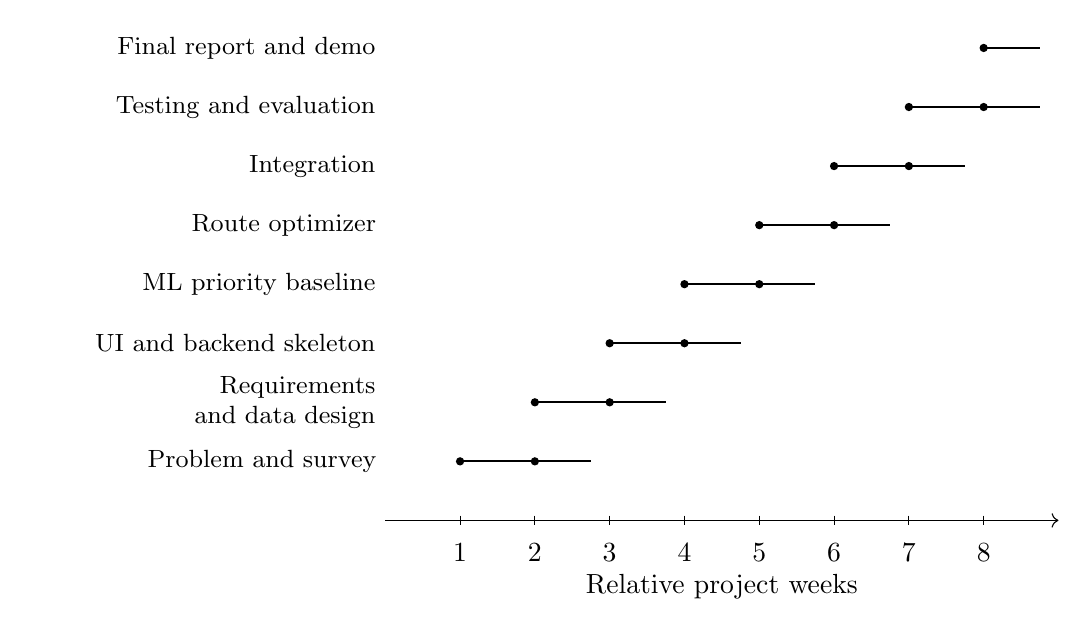
\begin{tikzpicture}[x=0.95cm,y=0.75cm]
\draw[->] (0,0)--(9,0);\node[below] at (4.5,-0.75) {Relative project weeks};
\foreach \x/\lab in {1/1,2/2,3/3,4/4,5/5,6/6,7/7,8/8} {\draw (\x,0.08)--(\x,-0.08) node[below=3pt]{\lab};}
\foreach \y/\name/\start/\end in {1/Problem and survey/1/2,2/Requirements and data design/2/3,3/UI and backend skeleton/3/4,4/ML priority baseline/4/5,5/Route optimizer/5/6,6/Integration/6/7,7/Testing and evaluation/7/8,8/Final report and demo/8/8} {
  \node[anchor=east,align=right,font=\small,text width=43mm] at (0,\y){\name};
  \draw[thick] (\start,\y)--(\end+0.75,\y);
  \foreach \x in {\start,...,\end} {\fill (\x,\y) circle (1.5pt);}
}
\end{tikzpicture}
\caption{Indicative dependency-aware project timeline (relative weeks, not calendar dates).}
\label{fig:gantt}
\end{figure}

\section{Task Network}
\begin{figure}[htbp]
\centering
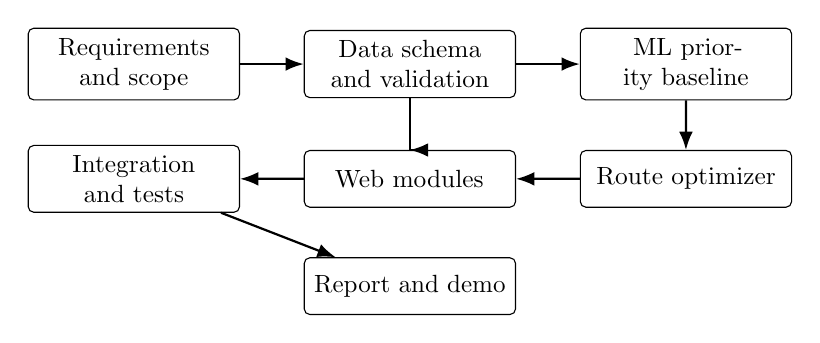
\begin{tikzpicture}[node distance=7mm and 9mm,scale=0.9,transform shape]
\node[block,text width=27mm] (req) {Requirements and scope};
\node[block,right=of req,text width=27mm] (data) {Data schema and validation};
\node[block,right=of data,text width=27mm] (ml) {ML priority baseline};
\node[block,below=of ml,text width=27mm] (route) {Route optimizer};
\node[block,left=of route,text width=27mm] (web) {Web modules};
\node[block,left=of web,text width=27mm] (test) {Integration and tests};
\node[block,below=of web,text width=27mm] (report) {Report and demo};
\draw[line] (req)--(data);\draw[line] (data)--(ml);\draw[line] (ml)--(route);\draw[line] (route)--(web);\draw[line] (web)--(test);\draw[line] (test)--(report);
\draw[line] (data.south) |- (web.north);
\end{tikzpicture}
\caption{Project task dependency network.}
\end{figure}

\chapter{SOFTWARE REQUIREMENTS SPECIFICATION}

\section{Introduction}
This Software Requirements Specification (SRS) defines the expected behaviour, interfaces, constraints, and quality attributes of the proposed application. It is intended to guide implementation and testing. Requirements are written in testable terms where possible; a requirement is not considered complete merely because a screen exists, it must also be checked with valid and invalid inputs.

\section{Project Scope}
The application is a browser-accessible planning tool for authorized MRs and managers. It stores master and event data, estimates visit priority, constructs route plans, and displays progress. It supports daily planning for a selected date and territory. It is not a prescribing system and does not require patient-level clinical data.

\section{User Classes and Characteristics}
\subsection{Medical Representative}
The MR works with an assigned territory and an assigned set of doctors. The MR needs to view the day's visits, understand priority and appointment constraints, generate or refresh a route, inspect travel and timing estimates, and update visit status and outcomes. The interface should be usable on a standard laptop browser and should avoid requiring the MR to understand optimization internals.

\subsection{Manager}
The manager monitors activity across representatives or territories permitted by the assigned role. Required views include planned, completed, pending, and high-priority visits; MR-wise activity; visit status; and route or summary reports. The manager may review or adjust planning inputs within authorized permissions but should not see data outside the permitted scope.

\subsection{Administrator or Authorized Maintainer}
An administrator manages account roles and configuration. Depending on the prototype implementation, this role may be restricted to seeded accounts and configuration tasks rather than exposed as a third full dashboard. Administrative actions must be logged and separated from normal MR actions.

\section{Assumptions and Dependencies}
\begin{itemize}[leftmargin=1.2cm]
\item Users have valid accounts and are assigned roles and territories before using operational views.
\item The master data uses stable internal identifiers for doctors and MRs.
\item Time zones, date formats, and time units are standardized across the frontend, backend, and database.
\item Travel-time and distance values can be supplied for all candidate arcs or an explicit fallback is available.
\item A supervised ML model is only trained if labels are sufficiently reliable; otherwise the application uses a declared baseline ranking.
\item The first prototype runs in a controlled environment and may use anonymized synthetic data.
\end{itemize}

\section{Functional Requirements}
\begin{longtable}{p{20mm}p{50mm}p{61mm}}
\caption{Functional requirements and acceptance checks.}\label{tab:functional-req}\\
\toprule
\textbf{ID} & \textbf{Requirement} & \textbf{Acceptance check}\\
\midrule
\endfirsthead
\toprule
\textbf{ID} & \textbf{Requirement} & \textbf{Acceptance check}\\
\midrule
\endhead
FR-01 & Authenticate users. & Valid credentials open the permitted view; invalid credentials do not grant access.\\
FR-02 & Enforce role-based permissions. & MR and manager accounts cannot access unauthorized screens or records through direct API calls.\\
FR-03 & Manage doctor master data. & Authorized users can create/read/update doctor fields; required fields and coordinates are validated.\\
FR-04 & Manage MR and territory data. & Working hours, territory, and start/end locations are stored and checked.\\
FR-05 & Manage visits and appointments. & Visits can be created, viewed, rescheduled, and assigned statuses with date and time constraints.\\
FR-06 & Validate data before model inference. & Missing and malformed values are reported or handled by documented rules.\\
FR-07 & Predict visit priority. & The service returns a class or score and model version for supported feature inputs.\\
FR-08 & Generate an optimized route. & The optimizer uses a time matrix, service duration, time windows, working hours, and priority-aware objective settings.\\
FR-09 & Report infeasible route requests. & The API returns a clear status without presenting a failed route as a valid schedule.\\
FR-10 & Display the MR dashboard. & The MR sees assigned daily visits, priority, route order, estimated times, and statuses.\\
FR-11 & Update visit outcomes. & Authorized visit status and follow-up fields are saved and reflected in the dashboard.\\
FR-12 & Display manager summaries. & Aggregates include planned/completed/pending visits and priority/activity summaries for authorized scope.\\
FR-13 & Refresh plans after changes. & A changed appointment marks a prior route stale or enables route regeneration.\\
FR-14 & Compare baseline and proposed plans. & The evaluation output records metrics for identical input instances.\\
FR-15 & Preserve auditable identifiers and timestamps. & Records use stable IDs and timestamps for relevant updates and generated plans.\\
\bottomrule
\end{longtable}

\section{External Interface Requirements}
\subsection{User Interfaces}
The system provides a login view, an MR dashboard, doctor/appointment views, route-generation controls, visit-status controls, and a manager dashboard. Status should be communicated with text as well as colour. A generated route should show priority, stop order, time-window information, and estimated travel, and should distinguish a confirmed plan from a stale or failed plan.

\subsection{Software Interfaces}
The React frontend calls FastAPI REST endpoints over HTTP(S). The backend accesses MySQL through a database client or ORM. The ML model is loaded by the backend as a versioned preprocessing/model pipeline. The routing component receives validated routing nodes, durations, a travel-time matrix, time windows, and solver configuration. External map APIs, if used, must be isolated behind an adapter so a controlled matrix can be substituted for tests.

\subsection{Hardware Interfaces}
No special embedded hardware is required. Standard developer or application-server hardware is sufficient for the prototype. A mobile GPS receiver is outside the initial implementation scope.

\subsection{Communication Interfaces}
Requests and responses use JSON over REST endpoints. Authentication tokens or secure sessions should be applied according to the deployment model. Request timeouts, input size limits, and error codes should be consistent, and sensitive content should not be written to plain-text logs.

\section{Non-Functional Requirements}
\subsection{Performance Requirements}
The system should return normal CRUD and dashboard requests within a practical interactive time under the supported prototype dataset. Route generation should have a configurable upper time limit. The system must record solver duration and distinguish a feasible solution from timeout or infeasibility. Exact thresholds should be finalized after the expected dataset size is known and measured on the target environment.

\subsection{Safety and Reliability Requirements}
The application must not imply that an estimated route guarantees a visit or that a predicted class is a definitive business decision. It should show uncertainty or model limitations when appropriate. Invalid or conflicting appointment windows should be flagged before route generation. A failed solver response must not overwrite a previous valid route without confirmation.

\subsection{Security Requirements}
Passwords must be hashed using a suitable password-hashing mechanism. Endpoints must validate authenticated identity and role. Database credentials and API keys must be stored outside source control. Data access must be restricted by user role and assigned territory. Inputs are validated server-side, errors avoid leaking secrets, and logs exclude credentials and unnecessary personally identifying information.

\subsection{Software Quality Attributes}
The software should be maintainable through separation of frontend, API, data access, ML, and optimization modules. Testability requires deterministic sample data and fixed test matrices. Usability requires clear status feedback. Portability should be supported by environment-based configuration. Reproducibility requires versioning of model artefacts, data preparation rules, and evaluation input sets.

\section{System Requirements}
\subsection{Database Requirements}
The relational database stores users/roles, doctor profiles, MR profiles, visits, appointments, priority predictions, routes, and route stops. Foreign-key integrity should be used where supported. Timestamps should be stored consistently. Historical visit data should be treated as append-only where possible, with controlled updates when correcting errors.

\subsection{Software Requirements}
The proposed stack is React.js, Python, FastAPI, scikit-learn, Google OR-Tools, and MySQL. The precise supported versions should be pinned in dependency files before integration and deployment. Browser support should be tested against the current browser used by the target users.

\subsection{Hardware Requirements}
A machine with a dual-core processor, at least 4 GB RAM, and adequate storage is proposed for local development. The optimizer may need additional CPU or memory for larger routing instances. Production capacity must be chosen only after workload tests.

\section{SDLC Model to Be Applied}
An iterative and incremental development model is suitable because the project contains separable modules with uncertain data and route behaviour. Each increment should produce a demonstrable component: first requirements and schema, then basic CRUD and authentication, then the ML baseline, then route generation, then dashboards and evaluation. Each increment includes tests and review. This is preferable to postponing integration until every module has been completed independently.

\begin{figure}[htbp]
\centering
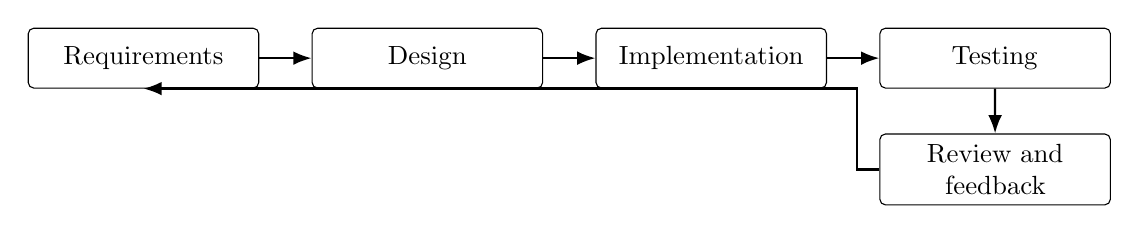
\begin{tikzpicture}[node distance=6mm and 7mm,scale=0.95,transform shape]
\node[block,text width=28mm] (req) {Requirements};
\node[block,right=of req,text width=28mm] (design) {Design};
\node[block,right=of design,text width=28mm] (build) {Implementation};
\node[block,right=of build,text width=28mm] (test) {Testing};
\node[block,below=of test,text width=28mm] (review) {Review and feedback};
\draw[line] (req)--(design);\draw[line] (design)--(build);\draw[line] (build)--(test);\draw[line] (test)--(review);
\draw[line] (review.west) -- ++(-3mm,0) |- (req.south);
\end{tikzpicture}
\caption{Iterative development model proposed for the prototype.}
\end{figure}

\section{System Implementation Plan}
Implementation should proceed by vertical slices so that each module is testable through the UI and API. The recommended sequence is: database schema and test fixtures; authentication and role checks; master data and appointment CRUD; priority service with a baseline model; route service and infeasibility handling; schedule and manager dashboards; then reproducible tests and evaluation. The route service should be built against a fixed synthetic travel matrix before it depends on a live routing provider.

\chapter{DETAILED DESIGN}

\section{Introduction}
This chapter describes the architecture, user behaviour, module boundaries, database entities, class relationships, and main runtime interactions. Diagrams are generated in TikZ to remain editable within this LaTeX source. They describe the proposed design and should be revised if the implementation changes.

\section{Architectural Design}
The design has five logical layers: presentation, API/application services, data preparation and ML inference, constraint and route optimization, and persistence. The frontend does not train models or solve routing directly. It sends requests to the backend, which validates the request, retrieves related records, invokes the appropriate service, stores relevant results, and returns a structured response.

\begin{figure}[htbp]
\centering
\resizebox{\textwidth}{!}{%
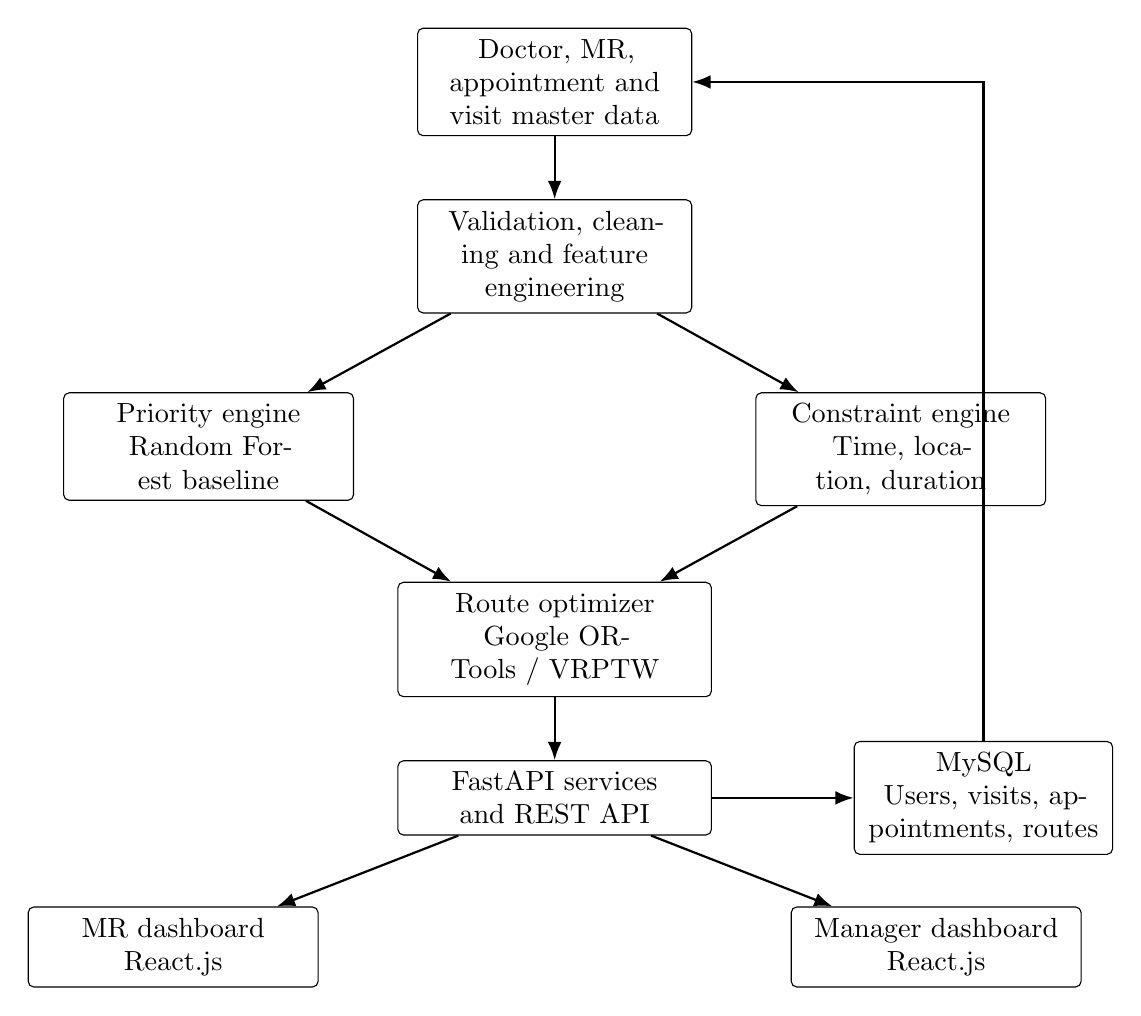
\begin{tikzpicture}[node distance=8mm and 8mm]
\node[block,text width=32mm] (master) {Doctor, MR, appointment and visit master data};
\node[block,below=of master,text width=32mm] (prep) {Validation, cleaning and feature engineering};
\node[block,below left=10mm and 8mm of prep,text width=34mm] (ml) {Priority engine\\Random Forest baseline};
\node[block,below right=10mm and 8mm of prep,text width=34mm] (constraint) {Constraint engine\\Time, location, duration};
\node[block,below=17mm of $(ml)!0.5!(constraint)$,text width=37mm] (route) {Route optimizer\\Google OR-Tools / VRPTW};
\node[block,below=of route,text width=37mm] (api) {FastAPI services and REST API};
\node[block,below left=9mm and 10mm of api,text width=34mm] (mr) {MR dashboard\\React.js};
\node[block,below right=9mm and 10mm of api,text width=34mm] (manager) {Manager dashboard\\React.js};
\node[block,right=18mm of api,text width=30mm] (db) {MySQL\\Users, visits, appointments, routes};
\draw[line] (master)--(prep);\draw[line] (prep)--(ml);\draw[line] (prep)--(constraint);
\draw[line] (ml)--(route);\draw[line] (constraint)--(route);\draw[line] (route)--(api);
\draw[line] (api)--(mr);\draw[line] (api)--(manager);
\draw[line] (api)--(db);\draw[line] (db.north) |- (master.east);
\end{tikzpicture}}
\caption{Overall system architecture.}
\label{fig:architecture}
\end{figure}

\subsection{Presentation Layer}
The presentation layer contains the login interface and role-specific dashboards. It is responsible for collecting user inputs, showing validation messages, displaying the daily route, and allowing authorized status updates. The client should not be trusted to enforce permissions; all important permission checks occur on the backend.

\subsection{Application and API Layer}
FastAPI endpoints coordinate user authentication, doctor and MR records, appointments, visit outcomes, priority inference, route generation, and dashboard summaries. Request and response schemas define the contract. Domain rules should be implemented in service functions rather than scattered throughout individual route handlers.

\subsection{Machine-Learning Layer}
The ML layer takes prepared features and returns a priority class or score. Preprocessing and the classifier should be saved together as a pipeline so inference receives the same transformations as training. Model version, training-data version, and timestamp should be associated with predictions. The model must not generate the route itself.

\subsection{Optimization Layer}
The optimization layer receives candidate locations, appointment windows, service durations, MR working time, the travel-time matrix, and optional priority penalties or rewards. It constructs a VRPTW model and searches for a feasible solution that minimizes the configured cost. It returns route stops, time estimates, objective components when available, solver status, and diagnostics. The system should distinguish infeasible input, timeout, and successful route generation.

\subsection{Persistence Layer}
MySQL stores operational entities and generated plans. The application should avoid storing full copies of derived information when a reference and version are sufficient. Records that support auditability, such as visit outcomes and route generation metadata, should retain timestamps and relevant status values.

\section{System Workflow and Data Flow}
The standard MR workflow begins at login. The MR chooses a date and territory, and the application retrieves assigned doctors and appointment constraints. The backend cleans and validates the inputs, obtains or constructs a travel-time matrix, estimates visit priority, runs optimization, and returns the schedule. The MR can inspect the result and update visit status. The manager view aggregates activity for authorized records.

\begin{figure}[htbp]
\centering
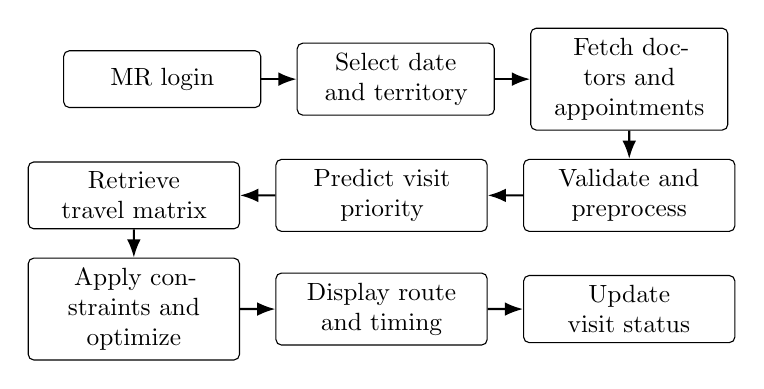
\begin{tikzpicture}[node distance=4mm and 5mm,scale=0.9,transform shape]
\node[block,text width=25mm] (login) {MR login};
\node[block,right=of login,text width=25mm] (date) {Select date and territory};
\node[block,right=of date,text width=25mm] (fetch) {Fetch doctors and appointments};
\node[block,below=of fetch,text width=27mm] (clean) {Validate and preprocess};
\node[block,left=of clean,text width=27mm] (predict) {Predict visit priority};
\node[block,left=of predict,text width=27mm] (matrix) {Retrieve travel matrix};
\node[block,below=of matrix,text width=27mm] (opt) {Apply constraints and optimize};
\node[block,right=of opt,text width=27mm] (display) {Display route and timing};
\node[block,right=of display,text width=27mm] (update) {Update visit status};
\draw[line] (login)--(date);\draw[line] (date)--(fetch);\draw[line] (fetch)--(clean);\draw[line] (clean)--(predict);\draw[line] (predict)--(matrix);\draw[line] (matrix)--(opt);\draw[line] (opt)--(display);\draw[line] (display)--(update);
\end{tikzpicture}
\caption{End-to-end MR data flow.}
\label{fig:dataflow}
\end{figure}

\section{UML Diagrams}
\subsection{Use Case Diagram}
The primary actors are the Medical Representative, Manager, and Administrator. The MR manages daily execution. The manager views permitted aggregate performance and route information. The administrator manages roles and configuration. Route generation includes retrieval, validation, priority prediction, constraint assembly, optimization, and persistence.

\begin{figure}[htbp]
\centering
\resizebox{\textwidth}{!}{%
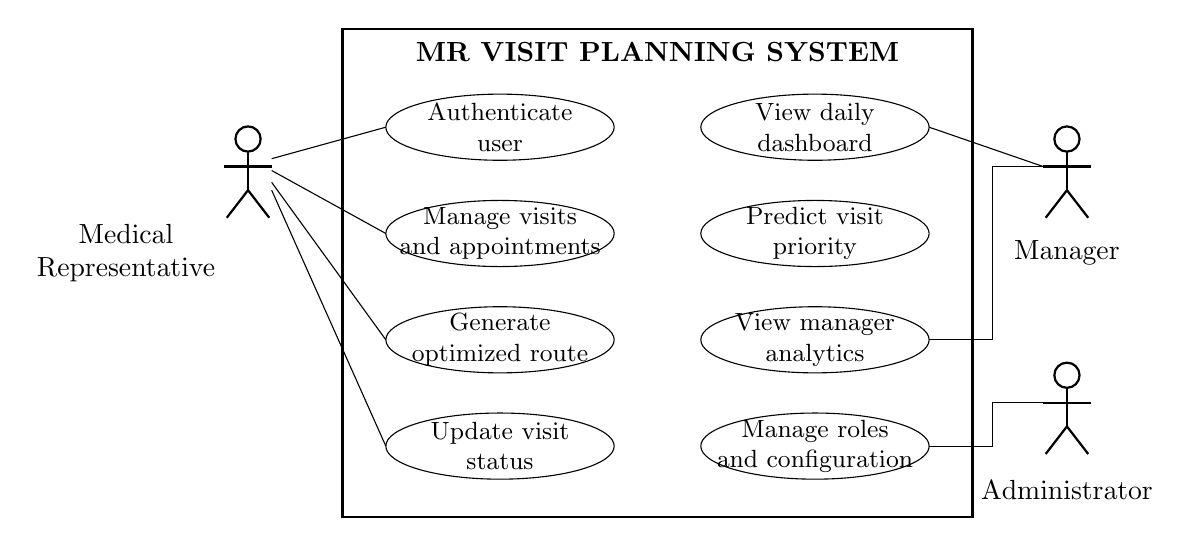
\begin{tikzpicture}[x=1cm,y=1cm]
% System boundary and title
\draw[thick] (2.0,0.4) rectangle (10.0,6.6);
\node[font=\bfseries] at (6.0,6.3) {MR VISIT PLANNING SYSTEM};
% Use cases: line-broken labels keep text inside the ellipses
\foreach \x/\y/\label in {4.0/5.35/a,8.0/5.35/b,4.0/4.0/c,8.0/4.0/d,4.0/2.65/e,8.0/2.65/f,4.0/1.3/g,8.0/1.3/h} {
  \draw (\x,\y) ellipse (1.45 and 0.42);
}
\node[align=center,font=\small] at (4.0,5.35) {Authenticate\\user};
\node[align=center,font=\small] at (8.0,5.35) {View daily\\dashboard};
\node[align=center,font=\small] at (4.0,4.0) {Manage visits\\and appointments};
\node[align=center,font=\small] at (8.0,4.0) {Predict visit\\priority};
\node[align=center,font=\small] at (4.0,2.65) {Generate\\optimized route};
\node[align=center,font=\small] at (8.0,2.65) {View manager\\analytics};
\node[align=center,font=\small] at (4.0,1.3) {Update visit\\status};
\node[align=center,font=\small] at (8.0,1.3) {Manage roles\\and configuration};
% Stick-figure actor: Medical Representative
\draw[thick] (0.8,5.2) circle (0.16);
\draw[thick] (0.8,5.04)--(0.8,4.55);
\draw[thick] (0.5,4.85)--(1.1,4.85);
\draw[thick] (0.8,4.55)--(0.53,4.2);
\draw[thick] (0.8,4.55)--(1.07,4.2);
\node[align=center] at (-0.75,3.75) {Medical\\Representative};
% Manager and administrator actors
\draw[thick] (11.2,5.2) circle (0.16);
\draw[thick] (11.2,5.04)--(11.2,4.55);
\draw[thick] (10.9,4.85)--(11.5,4.85);
\draw[thick] (11.2,4.55)--(10.93,4.2);
\draw[thick] (11.2,4.55)--(11.47,4.2);
\node[align=center] at (11.2,3.75) {Manager};
\draw[thick] (11.2,2.2) circle (0.16);
\draw[thick] (11.2,2.04)--(11.2,1.55);
\draw[thick] (10.9,1.85)--(11.5,1.85);
\draw[thick] (11.2,1.55)--(10.93,1.2);
\draw[thick] (11.2,1.55)--(11.47,1.2);
\node[align=center] at (11.2,0.75) {Administrator};
% Actor associations. Medical Representative connects to MR functions only.
\draw (1.1,4.95)--(2.55,5.35);
\draw (1.1,4.8)--(2.55,4.0);
\draw (1.1,4.65)--(2.55,2.65);
\draw (1.1,4.55)--(2.55,1.3);
% Manager connects to monitoring and analytics; administrator manages access/configuration.
\draw (9.45,5.35)--(10.9,4.85);
\draw (9.45,2.65)--(10.25,2.65)--(10.25,4.85)--(10.9,4.85);
\draw (10.9,1.85)--(10.25,1.85)--(10.25,1.3)--(9.45,1.3);
\end{tikzpicture}}
\caption{Use case UML diagram for the proposed application.}
\label{fig:usecase}
\end{figure}

\subsection{Activity Diagram: MR User Behaviour}
The activity diagram represents the behaviour visible to an MR. The user can review the suggested route before execution. If route generation fails, the system displays a reason and leaves the previous valid route intact. A visit is marked complete only after the MR records its status and any required outcome.

\begin{figure}[htbp]
\centering
\resizebox{0.86\textwidth}{!}{%
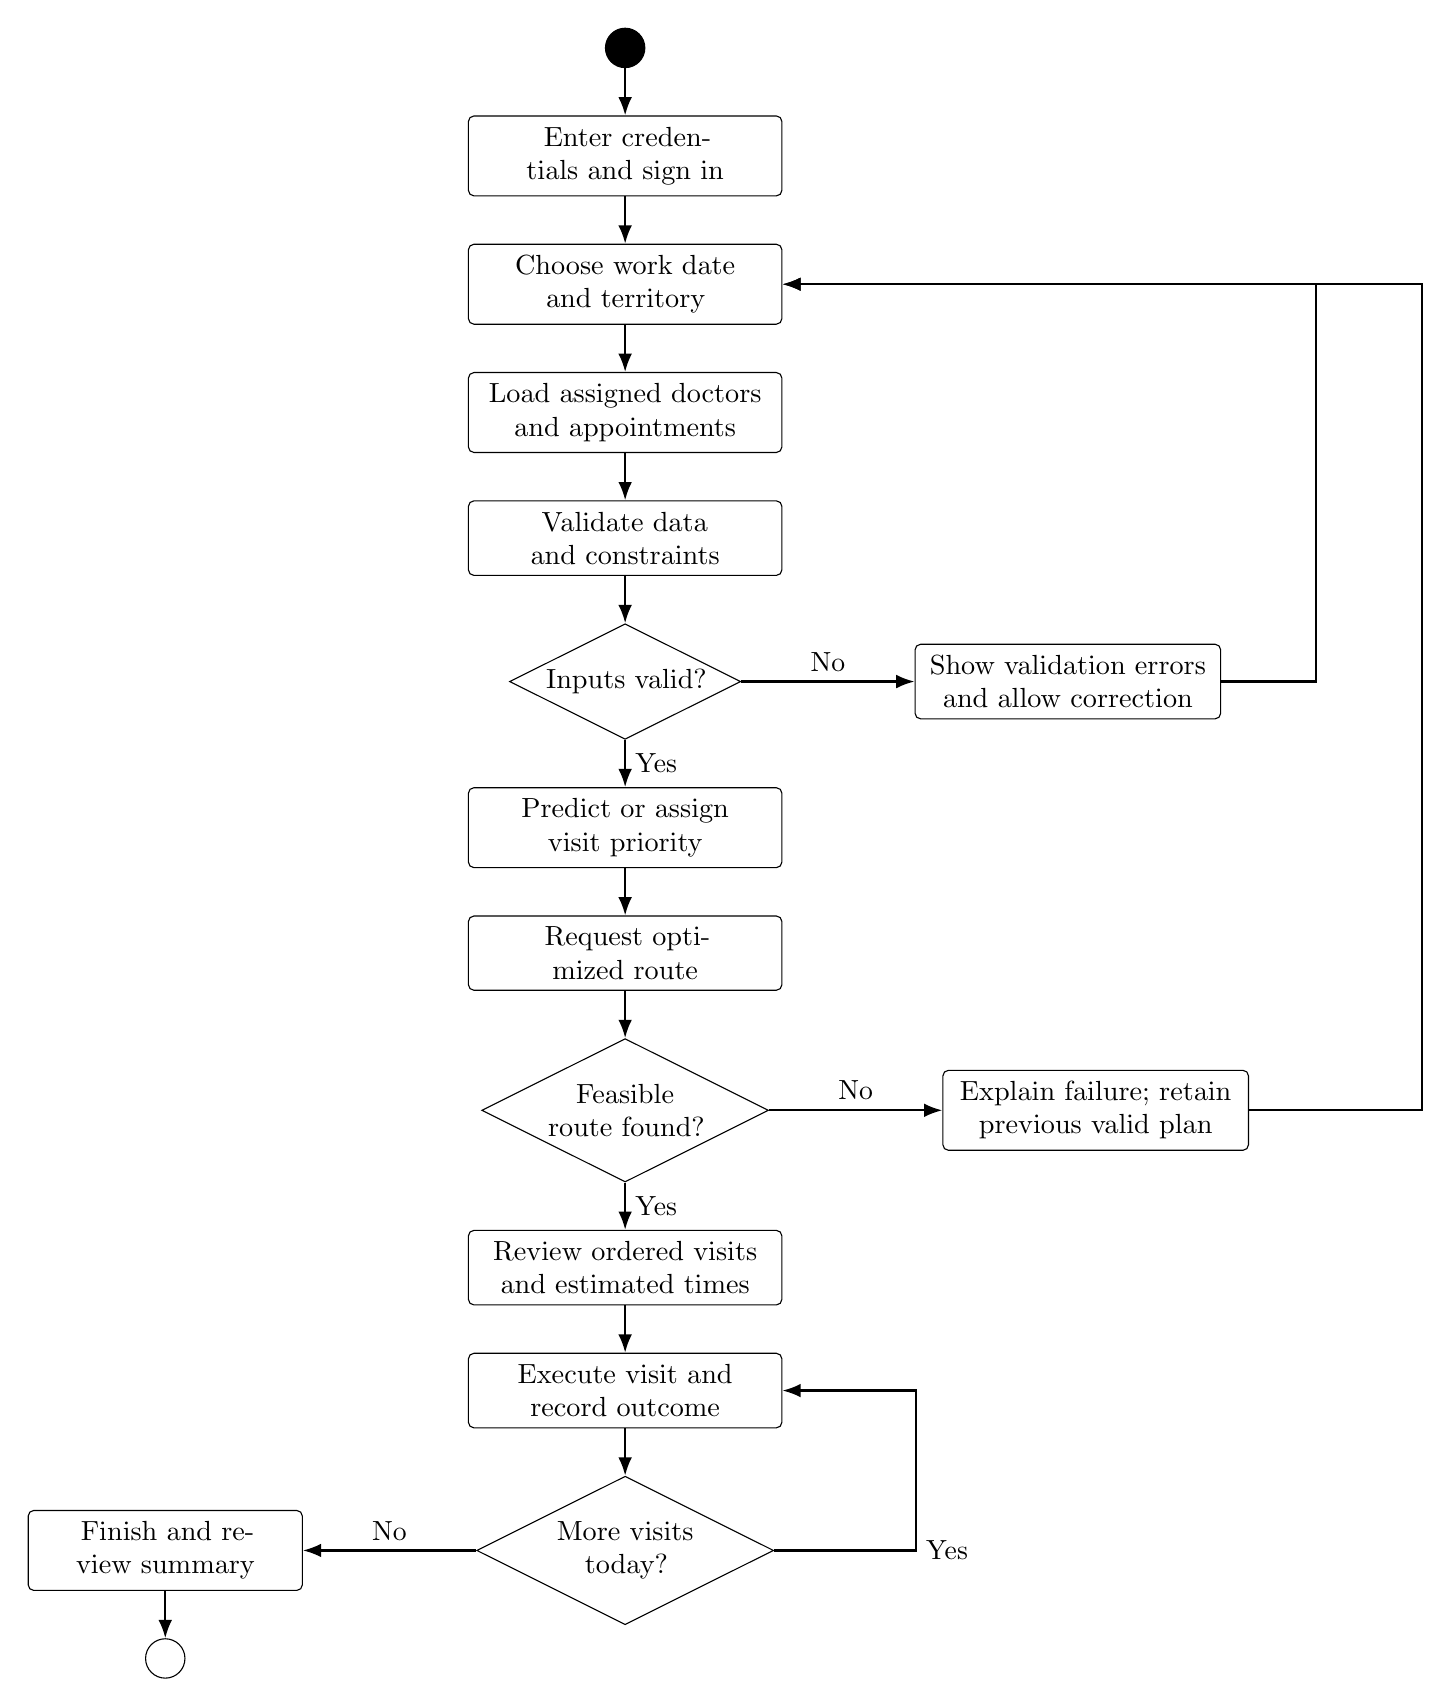
\begin{tikzpicture}[node distance=6mm]
\node[circle,draw,fill=black,minimum size=5mm,inner sep=0pt] (start) {};
\node[block,below=of start,text width=37mm] (signin) {Enter credentials and sign in};
\node[block,below=of signin,text width=37mm] (select) {Choose work date and territory};
\node[block,below=of select,text width=37mm] (fetch) {Load assigned doctors and appointments};
\node[block,below=of fetch,text width=37mm] (validate) {Validate data and constraints};
\node[decision,below=of validate] (valid) {Inputs valid?};
\node[block,right=22mm of valid,text width=36mm] (error) {Show validation errors and allow correction};
\node[block,below=of valid,text width=37mm] (priority) {Predict or assign visit priority};
\node[block,below=of priority,text width=37mm] (optimize) {Request optimized route};
\node[decision,below=of optimize] (routeok) {Feasible route found?};
\node[block,right=22mm of routeok,text width=36mm] (failed) {Explain failure; retain previous valid plan};
\node[block,below=of routeok,text width=37mm] (review) {Review ordered visits and estimated times};
\node[block,below=of review,text width=37mm] (visit) {Execute visit and record outcome};
\node[decision,below=of visit] (more) {More visits today?};
\node[block,left=22mm of more,text width=32mm] (finish) {Finish and review summary};
\node[circle,draw,below=of finish,minimum size=5mm,inner sep=0pt] (end) {};
\draw[line] (start)--(signin);\draw[line] (signin)--(select);\draw[line] (select)--(fetch);\draw[line] (fetch)--(validate);\draw[line] (validate)--(valid);
\draw[line] (valid.east)--node[above]{No}(error.west);\draw[line] (error.east) -- ++(12mm,0) |- (select.east);
\draw[line] (valid.south)--node[right]{Yes}(priority.north);\draw[line] (priority)--(optimize);\draw[line] (optimize)--(routeok);
\draw[line] (routeok.east)--node[above]{No}(failed.west);\draw[line] (failed.east) -- ++(22mm,0) |- (select.east);
\draw[line] (routeok.south)--node[right]{Yes}(review.north);\draw[line] (review)--(visit);\draw[line] (visit)--(more);
\draw[line] (more.west)--node[above]{No}(finish.east);\draw[line] (finish)--(end);
\draw[line] (more.east) -- ++(18mm,0) node[right]{Yes} |- (visit.east);
\end{tikzpicture}}
\caption{Activity UML diagram showing MR behaviour and exception paths.}
\label{fig:activity-mr}
\end{figure}

\subsection{Sequence Diagram: Route Generation}
The sequence diagram clarifies the runtime messages between the user interface, API, database, priority model, and optimizer. The backend validates the request and obtains the inputs before calling either computational module. A successful route is stored and returned; failures are returned as explicit statuses.

\begin{figure}[htbp]
\centering
\resizebox{\textwidth}{!}{%
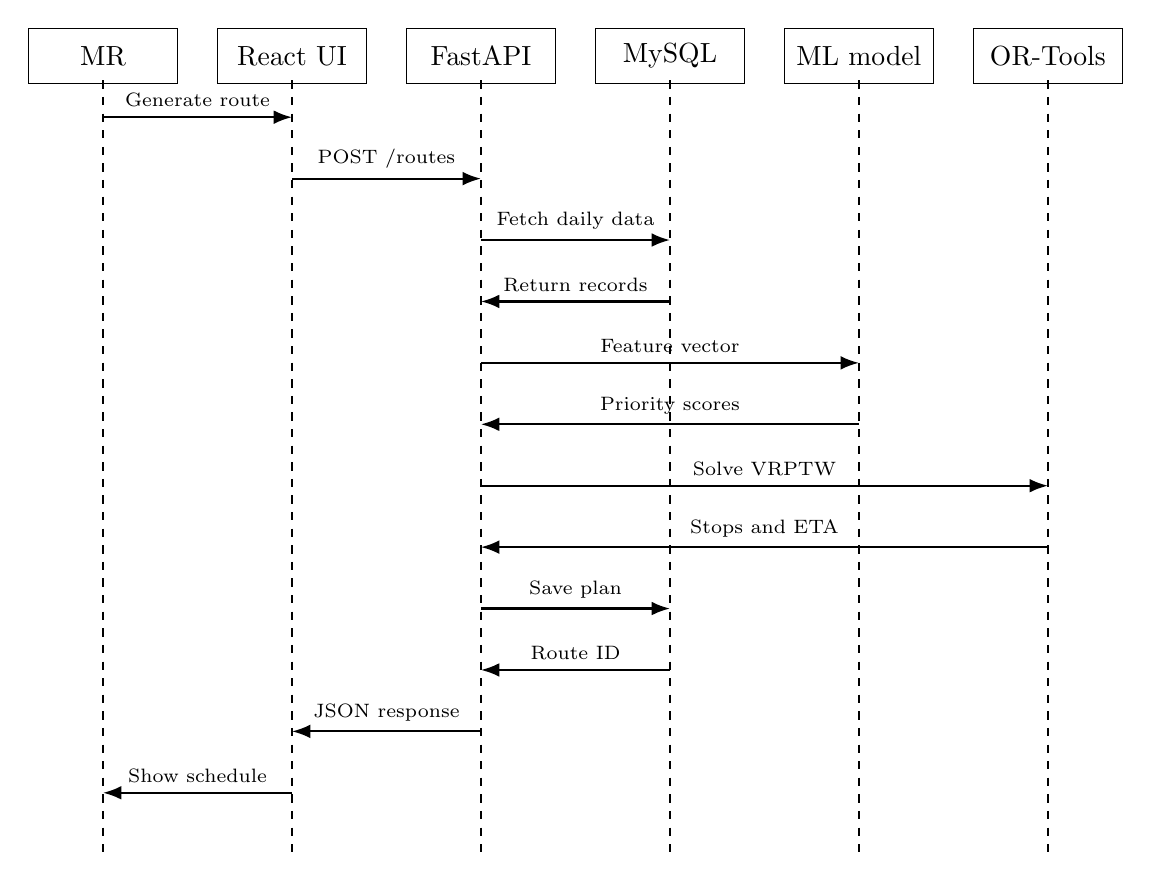
\begin{tikzpicture}[x=1cm,y=0.78cm]
\foreach \x/\name in {0/MR,2.4/React UI,4.8/FastAPI,7.2/MySQL,9.6/ML model,12/OR-Tools} {
  \node[draw,rectangle,minimum width=19mm,minimum height=7mm,align=center] at (\x,0) {\name};
  \draw[lifeline] (\x,-0.4)--(\x,-13.0);
}
\draw[line] (0,-1.0)--node[midway,above,font=\scriptsize]{Generate route}(2.4,-1.0);
\draw[line] (2.4,-2.0)--node[midway,above,font=\scriptsize]{POST /routes}(4.8,-2.0);
\draw[line] (4.8,-3.0)--node[midway,above,font=\scriptsize]{Fetch daily data}(7.2,-3.0);
\draw[line] (7.2,-4.0)--node[midway,above,font=\scriptsize]{Return records}(4.8,-4.0);
\draw[line] (4.8,-5.0)--node[midway,above,font=\scriptsize]{Feature vector}(9.6,-5.0);
\draw[line] (9.6,-6.0)--node[midway,above,font=\scriptsize]{Priority scores}(4.8,-6.0);
\draw[line] (4.8,-7.0)--node[midway,above,font=\scriptsize]{Solve VRPTW}(12,-7.0);
\draw[line] (12,-8.0)--node[midway,above,font=\scriptsize]{Stops and ETA}(4.8,-8.0);
\draw[line] (4.8,-9.0)--node[midway,above,font=\scriptsize]{Save plan}(7.2,-9.0);
\draw[line] (7.2,-10.0)--node[midway,above,font=\scriptsize]{Route ID}(4.8,-10.0);
\draw[line] (4.8,-11.0)--node[midway,above,font=\scriptsize]{JSON response}(2.4,-11.0);
\draw[line] (2.4,-12.0)--node[midway,above,font=\scriptsize]{Show schedule}(0,-12.0);
\end{tikzpicture}}
\caption{Sequence UML diagram for optimized route generation.}
\label{fig:sequence}
\end{figure}

\subsection{Class Diagram}
The class diagram gives the principal conceptual entities. It is not a literal ORM schema; implementation may split user roles into linked profile tables or use database-specific naming. The purpose is to establish identifiers, attributes, and associations before implementing the database.

\begin{figure}[htbp]
\centering
\resizebox{\textwidth}{!}{%
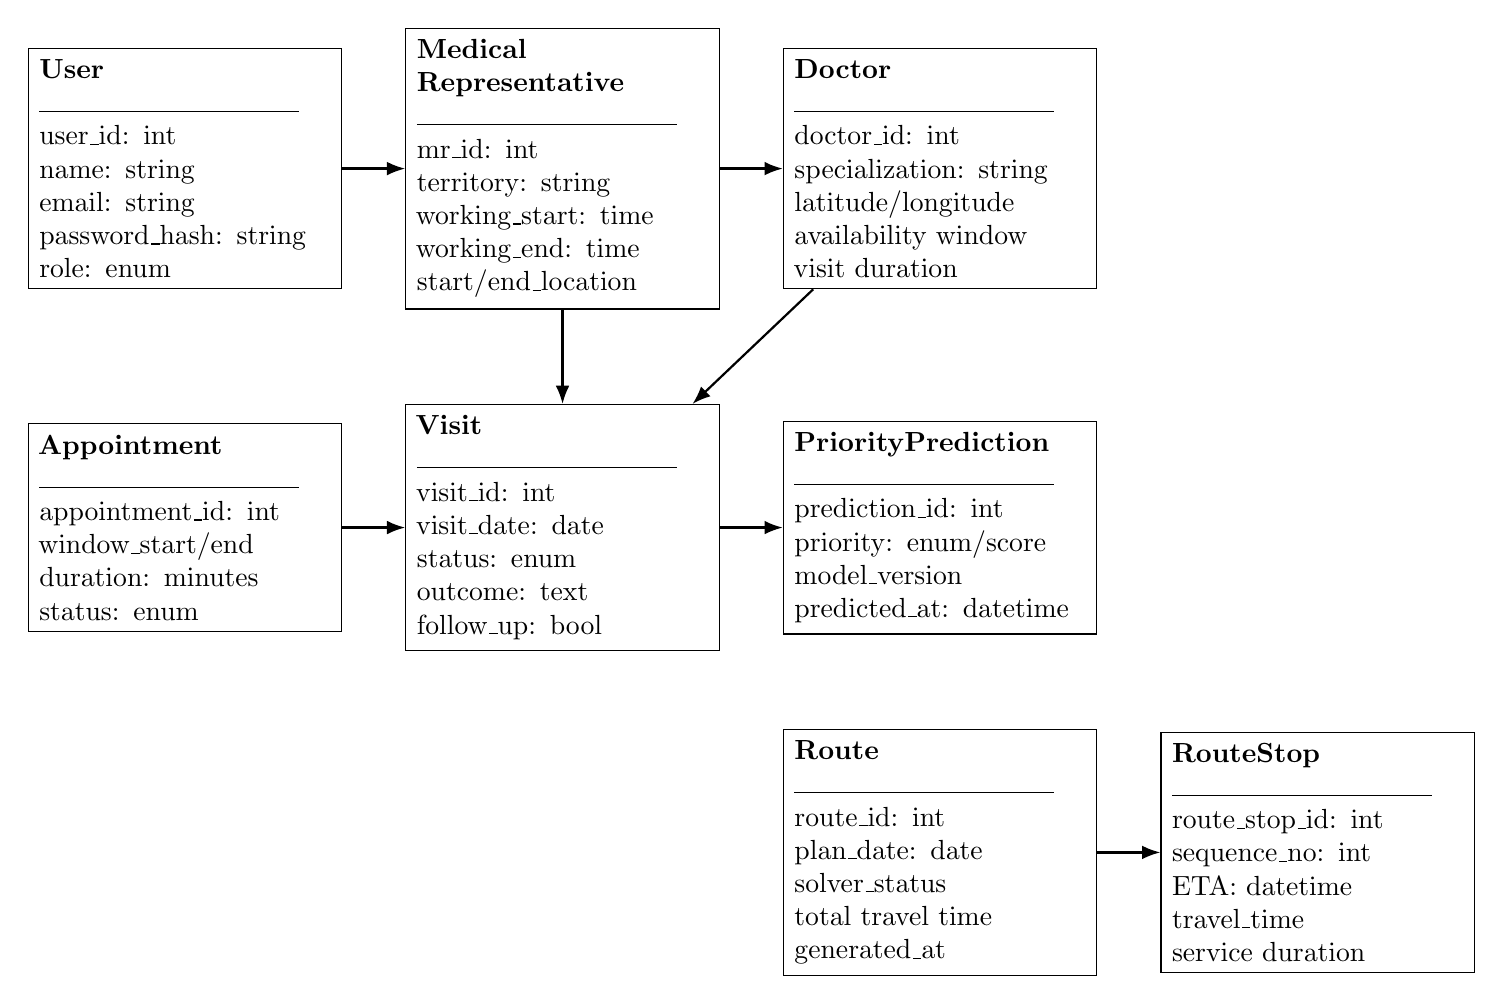
\begin{tikzpicture}[node distance=12mm and 8mm]
\node[umlclass] (user) {\textbf{User}\\\rule{33mm}{0.3pt}\\user\_id: int\\name: string\\email: string\\password\_hash: string\\role: enum};
\node[umlclass,right=of user] (mr) {\textbf{Medical\\Representative}\\\rule{33mm}{0.3pt}\\mr\_id: int\\territory: string\\working\_start: time\\working\_end: time\\start/end\_location};
\node[umlclass,right=of mr] (doctor) {\textbf{Doctor}\\\rule{33mm}{0.3pt}\\doctor\_id: int\\specialization: string\\latitude/longitude\\availability window\\visit duration};
\node[umlclass,below=of mr] (visit) {\textbf{Visit}\\\rule{33mm}{0.3pt}\\visit\_id: int\\visit\_date: date\\status: enum\\outcome: text\\follow\_up: bool};
\node[umlclass,left=of visit] (appointment) {\textbf{Appointment}\\\rule{33mm}{0.3pt}\\appointment\_id: int\\window\_start/end\\duration: minutes\\status: enum};
\node[umlclass,right=of visit] (prediction) {\textbf{PriorityPrediction}\\\rule{33mm}{0.3pt}\\prediction\_id: int\\priority: enum/score\\model\_version\\predicted\_at: datetime};
\node[umlclass,below=of prediction] (route) {\textbf{Route}\\\rule{33mm}{0.3pt}\\route\_id: int\\plan\_date: date\\solver\_status\\total travel time\\generated\_at};
\node[umlclass,right=of route] (stop) {\textbf{RouteStop}\\\rule{33mm}{0.3pt}\\route\_stop\_id: int\\sequence\_no: int\\ETA: datetime\\travel\_time\\service duration};
\draw[relation] (user)--(mr);
\draw[relation] (mr)--(doctor);
\draw[relation] (doctor)--(visit);
\draw[relation] (mr)--(visit);
\draw[relation] (appointment)--(visit);
\draw[relation] (visit)--(prediction);
% MR-to-route foreign-key association is shown explicitly in the ER diagram (Figure~\ref{fig:er-diagram}).
\draw[relation] (route)--(stop);
% Doctor-to-route-stop association is represented in the ER diagram to avoid a crossing line.
\end{tikzpicture}}
\caption{Conceptual UML class diagram.}
\label{fig:class-diagram}
\end{figure}

\subsection{Entity--Relationship Diagram}
The ER view emphasizes keys and relationships for persistent storage. A doctor can be associated with multiple appointments and visits. An MR can perform many visits and generate multiple daily route plans. A route contains an ordered set of route stops. A priority prediction is associated with a visit and should retain the model version used to generate it.

\begin{figure}[htbp]
\centering
\resizebox{\textwidth}{!}{%
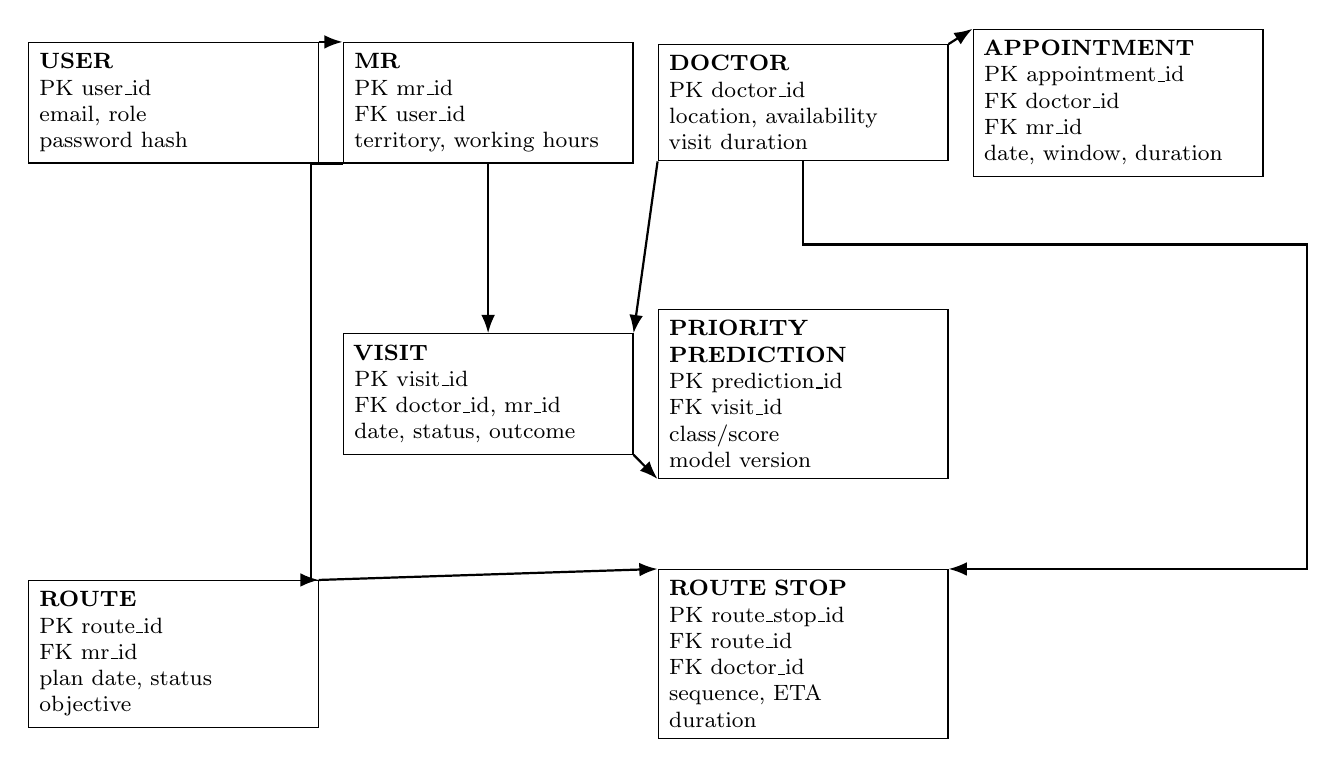
\begin{tikzpicture}[x=1cm,y=1cm]
\node[entity] (user) at (0,5.0) {\textbf{USER}\\PK user\_id\\email, role\\password hash};
\node[entity] (mr) at (4.0,5.0) {\textbf{MR}\\PK mr\_id\\FK user\_id\\territory, working hours};
\node[entity] (doctor) at (8.0,5.0) {\textbf{DOCTOR}\\PK doctor\_id\\location, availability\\visit duration};
\node[entity] (appt) at (12.0,5.0) {\textbf{APPOINTMENT}\\PK appointment\_id\\FK doctor\_id\\FK mr\_id\\date, window, duration};
\node[entity] (visit) at (4.0,1.3) {\textbf{VISIT}\\PK visit\_id\\FK doctor\_id, mr\_id\\date, status, outcome};
\node[entity] (pred) at (8.0,1.3) {\textbf{PRIORITY\\PREDICTION}\\PK prediction\_id\\FK visit\_id\\class/score\\model version};
\node[entity] (route) at (0.0,-2.0) {\textbf{ROUTE}\\PK route\_id\\FK mr\_id\\plan date, status\\objective};
\node[entity] (stop) at (8.0,-2.0) {\textbf{ROUTE STOP}\\PK route\_stop\_id\\FK route\_id\\FK doctor\_id\\sequence, ETA\\duration};
% Core relationships are routed through corners or whitespace to keep attributes legible.
\draw[line] (user.north east)--(mr.north west);
\draw[line] (mr.south)--(visit.north);
\draw[line] (doctor.south west)--(visit.north east);
\draw[line] (doctor.north east)--(appt.north west);
\draw[line] (visit.south east)--(pred.south west);
\draw[line] (mr.south west) -- ++(-4mm,0) |- (route.north east);
\draw[line] (route.north east)--(stop.north west);
\draw[line] (doctor.south) -- (8,3.2) -- (14.4,3.2) -- (14.4,0) |- (stop.north east);
\end{tikzpicture}}
\caption{Conceptual entity--relationship diagram.}
\label{fig:er-diagram}
\end{figure}

\subsection{State Diagram: Route Lifecycle}
A generated route has a lifecycle independent of visit statuses. It is initially a draft request, then either fails validation, is optimized and stored, becomes stale after an input changes, or is superseded by a regenerated route. Separating these states prevents the interface from treating a route produced with outdated appointment information as current.

\begin{figure}[htbp]
\centering
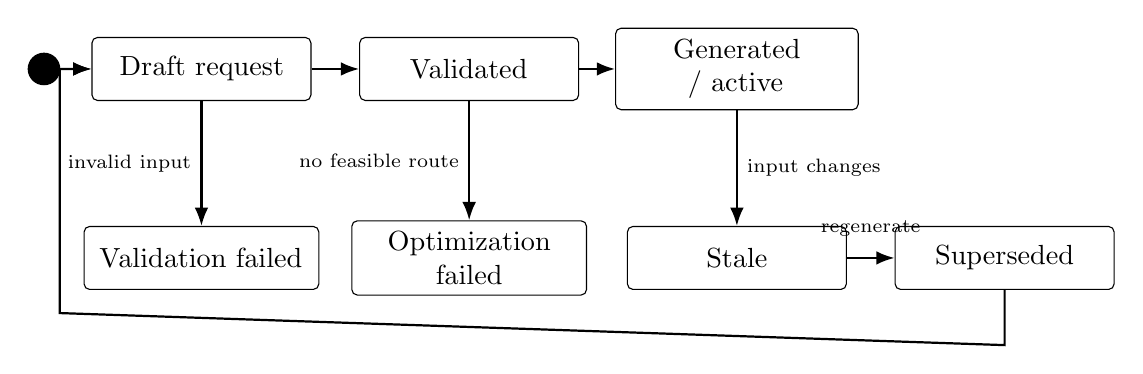
\begin{tikzpicture}[x=1cm,y=1cm]
\node[circle,draw,fill=black,minimum size=4mm,inner sep=0pt] (start) at (-1.0,3.0) {};
\node[block,text width=25mm] (draft) at (1.0,3.0) {Draft request};
\node[block,text width=25mm] (validated) at (4.4,3.0) {Validated};
\node[block,text width=28mm] (active) at (7.8,3.0) {Generated / active};
\node[block,text width=27mm] (invalid) at (1.0,0.6) {Validation failed};
\node[block,text width=27mm] (optfail) at (4.4,0.6) {Optimization failed};
\node[block,text width=25mm] (stale) at (7.8,0.6) {Stale};
\node[block,text width=25mm] (superseded) at (11.2,0.6) {Superseded};
\draw[line] (start)--(draft);
\draw[line] (draft)--(validated);
\draw[line] (validated)--(active);
\draw[line] (draft.south)--node[left,font=\scriptsize]{invalid input}(invalid.north);
\draw[line] (validated.south)--node[left,font=\scriptsize]{no feasible route}(optfail.north);
\draw[line] (active.south)--node[right,font=\scriptsize]{input changes}(stale.north);
\draw[line] (stale.east)--node[above,font=\scriptsize,yshift=4pt]{regenerate}(superseded.west);
\draw[line] (superseded.south) -- ++(0,-0.7) -- (-0.8,-0.1) -- (-0.8,3.0) -- (draft.west);
\end{tikzpicture}
\caption{State UML diagram for the route lifecycle.}
\label{fig:state-route}
\end{figure}

\subsection{Component Diagram}
The component view defines the principal software modules and their interfaces. The ML and optimizer are separate services at the logical level even if both are deployed inside the same backend process for the prototype.

\begin{figure}[htbp]
\centering
\resizebox{\textwidth}{!}{%
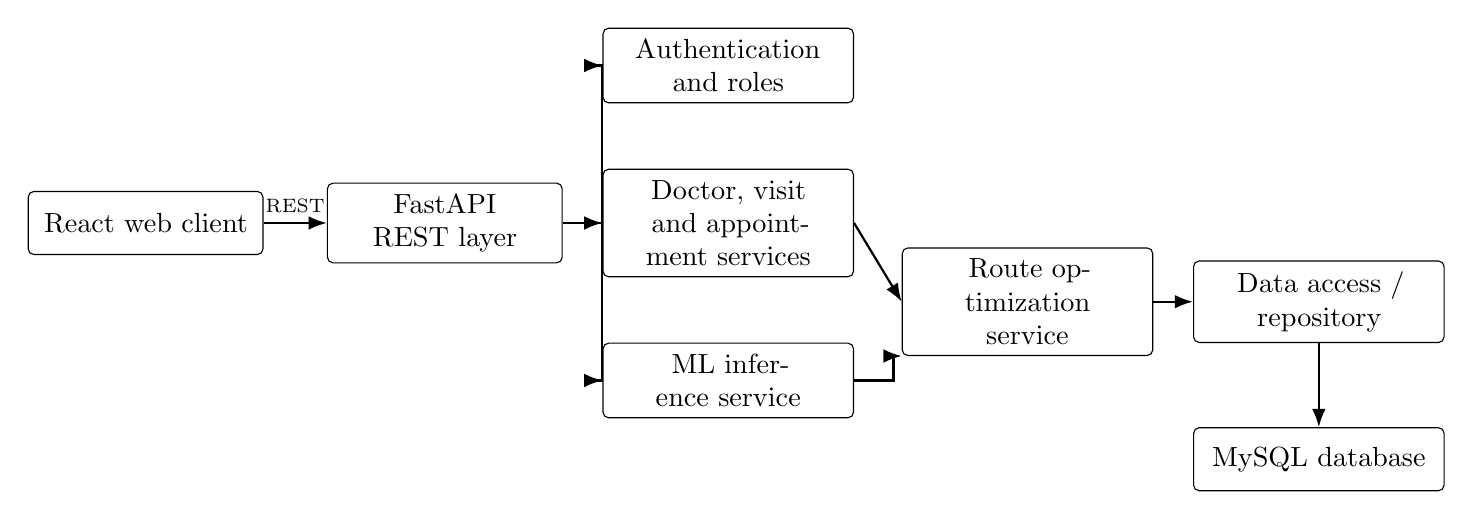
\begin{tikzpicture}[x=1cm,y=1cm]
\node[block,text width=27mm] (ui) at (0,2.0) {React web client};
\node[block,text width=27mm] (api) at (3.8,2.0) {FastAPI REST layer};
\node[block,text width=29mm] (auth) at (7.4,4.0) {Authentication and roles};
\node[block,text width=29mm] (domain) at (7.4,2.0) {Doctor, visit and appointment services};
\node[block,text width=29mm] (ml) at (7.4,0.0) {ML inference service};
\node[block,text width=29mm] (opt) at (11.2,1.0) {Route optimization\\service};
\node[block,text width=29mm] (repo) at (14.9,1.0) {Data access /\\repository};
\node[block,text width=29mm] (db) at (14.9,-1.0) {MySQL database};
\draw[line] (ui)--node[above,font=\scriptsize]{REST}(api);
\draw[line] (api.east) -- ++(5mm,0) |- (auth.west);
\draw[line] (api)--(domain);
\draw[line] (api.east) -- ++(5mm,0) |- (ml.west);
\draw[line] (domain.east)--(opt.west);
\draw[line] (ml.east) -- ++(5mm,0) |- (opt.south west);
\draw[line] (opt)--(repo);
% Persistence is provided by the repository component; domain-to-repository dependency is abstracted through the API layer.
\draw[line] (repo.south)--(db.north);
\end{tikzpicture}}
\caption{Component diagram of the proposed software modules.}
\end{figure}

\subsection{Deployment Diagram}
For the prototype, the browser runs on a user device and communicates with the application backend over a network. The backend communicates with MySQL and invokes the ML and optimization libraries in the server environment. A future production deployment may separate these components into containers or independent services after measured load justifies it.

\begin{figure}[htbp]
\centering
\resizebox{\textwidth}{!}{%
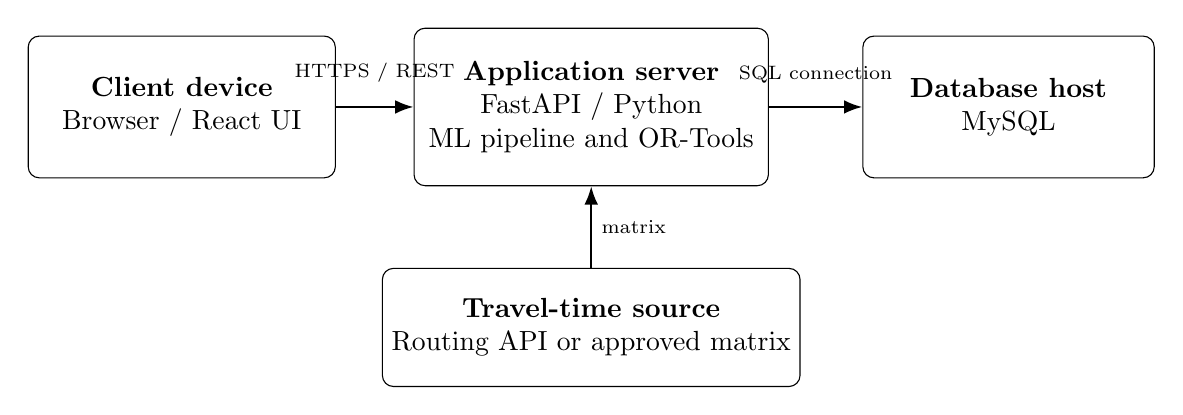
\begin{tikzpicture}[x=1cm,y=1cm]
\node[draw,rectangle,rounded corners,minimum width=39mm,minimum height=18mm,align=center] (client) at (0,1.8) {\textbf{Client device}\\Browser / React UI};
\node[draw,rectangle,rounded corners,minimum width=45mm,minimum height=20mm,align=center] (server) at (5.2,1.8) {\textbf{Application server}\\FastAPI / Python\\ML pipeline and OR-Tools};
\node[draw,rectangle,rounded corners,minimum width=37mm,minimum height=18mm,align=center] (db) at (10.5,1.8) {\textbf{Database host}\\MySQL};
\node[draw,rectangle,rounded corners,minimum width=45mm,minimum height=15mm,align=center] (map) at (5.2,-1.0) {\textbf{Travel-time source}\\Routing API or approved matrix};
\draw[line] (client.east)--node[midway,above=5pt,font=\scriptsize]{HTTPS / REST}(server.west);
\draw[line] (server.east)--node[midway,above=5pt,font=\scriptsize]{SQL connection}(db.west);
\draw[line] (map.north)--node[right,font=\scriptsize]{matrix}(server.south);
\end{tikzpicture}}
\caption{Deployment diagram for the academic prototype.}
\end{figure}

\subsection{Data Design}
The principal entities and proposed attributes are listed below. Exact column types and normalization choices should be verified during implementation.
\begin{longtable}{p{32mm}p{91mm}}
\caption{Proposed core data entities.}\label{tab:data-entities}\\
\toprule
\textbf{Entity} & \textbf{Important attributes}\\
\midrule
\endfirsthead
\toprule
\textbf{Entity} & \textbf{Important attributes}\\
\midrule
\endhead
Doctor & doctor\_id, specialization, territory, latitude, longitude, availability\_start, availability\_end, typical\_visit\_duration, priority\_category.\\
Medical Representative & mr\_id, user\_id, territory, working\_start, working\_end, start\_location, end\_location.\\
Visit & visit\_id, doctor\_id, mr\_id, visit\_date, planned\_time, actual\_arrival, actual\_departure, visit\_status, visit\_outcome, follow\_up\_required.\\
Appointment & appointment\_id, doctor\_id, mr\_id, appointment\_date, window\_start, window\_end, duration, status.\\
Priority Prediction & prediction\_id, visit\_id, priority\_class or score, model\_version, predicted\_at.\\
Route & route\_id, mr\_id, plan\_date, solver\_status, total\_travel\_time, total\_distance, generated\_at, model/config version.\\
Route Stop & route\_stop\_id, route\_id, doctor\_id, sequence\_number, estimated\_arrival, estimated\_departure, travel\_time, service\_duration.\\
User & user\_id, display\_name, email, password\_hash, role, active\_flag, created\_at.\\
\bottomrule
\end{longtable}

\subsection{Internal, Global, and Temporary Data Structures}
Internal data structures include validated feature frames for ML inference, route nodes, a travel-time matrix, time-window arrays, and solver results. Global reference data includes doctor and MR identifiers, territory definitions, and allowed visit statuses. Temporary data may include a prediction batch, route candidate graph, and diagnostic messages while generating a plan. Temporary data should not be persisted unnecessarily, while outputs needed for audit and comparison should be saved with version metadata.

\subsection{Database Description and Integrity Rules}
Doctor and MR identifiers should be primary keys. Appointments reference both the relevant doctor and the assigned MR. Visits reference the doctor and MR and may reference an appointment. A priority prediction references the visit and model version. A route references the MR and plan date, and its ordered route-stop records reference the route and doctor. The schema should prohibit invalid foreign keys and define how deletion works; historical visits should normally be retained rather than cascade-deleted when a doctor record is deactivated.

\section{Machine-Learning Priority Model Design}
\subsection{Feature Set}
Potential features include historical visit frequency, days since last visit, previous visit outcome, follow-up requirement, existing priority category, appointment status, doctor engagement indicator, territory, and aggregate visit history. Features must be available at planning time. Any feature that reveals a future outcome or includes information recorded only after the planned visit would cause target leakage and should be excluded.

\subsection{Preprocessing and Training}
Preprocessing begins by checking identifiers, resolving duplicates, handling missing values with documented rules, validating categorical values, and checking time and location ranges. A train/test split should be created at the appropriate unit to avoid information leakage. If multiple rows belong to the same doctor or repeated planning period, the team should consider a grouped or time-aware split rather than randomly distributing nearly identical records across training and testing.

\begin{figure}[htbp]
\centering
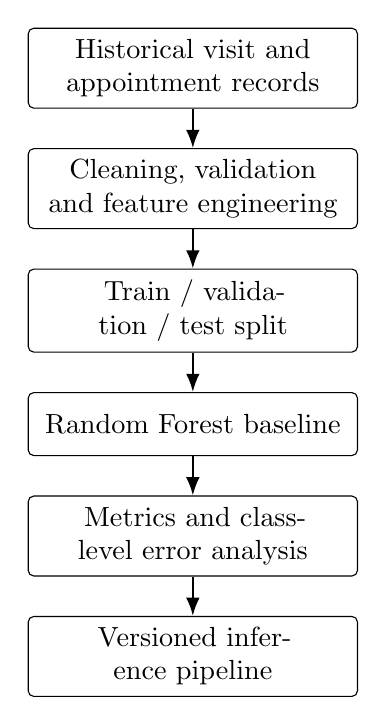
\begin{tikzpicture}[node distance=5mm]
\node[block,text width=39mm] (raw) {Historical visit and appointment records};
\node[block,below=of raw,text width=39mm] (clean) {Cleaning, validation and feature engineering};
\node[block,below=of clean,text width=39mm] (split) {Train / validation / test split};
\node[block,below=of split,text width=39mm] (train) {Random Forest baseline};
\node[block,below=of train,text width=39mm] (eval) {Metrics and class-level error analysis};
\node[block,below=of eval,text width=39mm] (serve) {Versioned inference pipeline};
\draw[line] (raw)--(clean);\draw[line] (clean)--(split);\draw[line] (split)--(train);\draw[line] (train)--(eval);\draw[line] (eval)--(serve);
\end{tikzpicture}
\caption{Proposed priority-prediction workflow.}
\label{fig:ml-pipeline}
\end{figure}

\subsection{Random Forest Formulation}
A Random Forest combines multiple decision trees. If the trained model contains $T$ trees and each tree returns a class prediction $h_t(\mathbf{x})$, the classification output can be expressed as a majority vote:
\begin{equation}
\hat{y}(\mathbf{x}) = \operatorname{mode}\{h_1(\mathbf{x}),h_2(\mathbf{x}),\ldots,h_T(\mathbf{x})\}.
\end{equation}
When calibrated class probabilities are available, a priority score could be defined as the probability of a designated class or as a business-approved weighted combination of class probabilities. The weighting must be specified with domain guidance, and it should not be selected only to make evaluation results look better.

\subsection{Prediction Output and Fallback}
The initial output classes are High, Medium, and Low, reflecting the illustrative categories in the review presentation. The final label schema must be aligned with the data source. If the agency has no reliable labels, a documented rule-based ranking using follow-up status, days since last visit, and appointment constraints can serve as a baseline. Such a ranking must be identified as rules-based and must not be described as a trained machine-learning result.

\section{Route Optimization Design}
\subsection{VRPTW Definition}
Let $V$ be the set of nodes containing the MR start location, candidate doctor visits, and the end location. For each feasible arc $(i,j)$, let $t_{ij}$ be estimated travel time and $d_{ij}$ be distance. Each doctor visit $i$ has a service duration $s_i$ and a hard or soft time window $[a_i,b_i]$. A planned route must respect the MR's working horizon and travel/service durations. If there are multiple MRs, the model becomes a multi-vehicle routing problem.

\subsection{Illustrative Objective}
A simplified objective is to minimize a weighted sum of travel time, waiting time, and penalties for unserved important visits:
\begin{equation}
\min Z = w_t\sum_{i\in V}\sum_{j\in V} t_{ij}x_{ij} + w_w\sum_{i\in V} W_i + \sum_{i\in V} w_u(p_i)u_i,
\label{eq:objective}
\end{equation}
where $x_{ij}$ indicates whether the route travels from node $i$ to node $j$, $W_i$ denotes waiting time, and $u_i$ indicates that visit $i$ is unserved. The penalty $w_u(p_i)$ can be larger for higher-priority visits, provided the project defines and validates that policy. This is a conceptual objective; exact variables and constraints depend on whether all visits are mandatory and whether time windows are hard or soft.

Important constraints include:
\begin{align}
&\text{Flow conservation:} && \sum_j x_{ij} = \sum_j x_{ji} \quad \text{for each intermediate node } i,\\
&\text{Visit coverage:} && \sum_j x_{ij} + u_i = 1 \quad \text{for each candidate visit } i,\\
&\text{Time propagation:} && T_j \geq T_i+s_i+t_{ij}-M(1-x_{ij}),\\
&\text{Time windows:} && a_i \leq T_i \leq b_i \quad \text{for mandatory hard-window visits},\\
&\text{Work horizon:} && H_{\text{start}} \leq T_i \text{ and route end} \leq H_{\text{end}}.
\end{align}
The large constant $M$ is a modelling device for conditional time propagation. A practical implementation should use solver dimensions and domain bounds where possible rather than an unnecessarily large arbitrary constant.

\subsection{Illustrative Appointment Inputs}
\begin{table}[htbp]
\centering
\begin{tabular}{c c c}
\toprule
\textbf{Doctor} & \textbf{Illustrative priority} & \textbf{Time window}\\
\midrule
A & High & 09:00--10:00\\
B & Medium & 10:00--12:00\\
C & High & 13:00--14:00\\
D & Low & 14:00--17:00\\
\bottomrule
\end{tabular}
\caption{Illustrative inputs from the design presentation; not experimental results.}
\label{tab:illustrative-doctors}
\end{table}

A high-priority visit can be scheduled later if its available time window requires it. A feasible schedule must account for travel and service time between all stops. The final stop order cannot be inferred from priority alone; it must be computed from the complete time and distance matrix, visit durations, windows, working hours, and objective weights.

\subsection{Travel-Time Matrix}
The optimizer requires a matrix of travel-time estimates, and optionally a distance matrix. The matrix may come from an approved routing API, agency-provided information, precomputed distances, or a clearly labelled controlled simulation. In experiments, the same matrix must be used when comparing baseline and proposed routes. If live traffic is unavailable, travel-time results must be described as estimated rather than real-time.

\subsection{Infeasibility Handling}
Before optimization, the backend should validate non-empty candidate sets, all required time windows, non-negative service durations, MR working hours, and matrix dimensions. When a route cannot be generated, the system should record solver status and show an understandable message. It may identify restrictive inputs, but it should not silently discard a visit or violate a hard window. Any optional-visit or soft-window policy must be explicit in the request configuration.

\section{Module Design}
\begin{longtable}{c p{40mm} p{72mm}}
\caption{Functional module breakdown.}\label{tab:modules}\\
\toprule
\textbf{No.} & \textbf{Module} & \textbf{Responsibilities}\\
\midrule
\endfirsthead
\toprule
\textbf{No.} & \textbf{Module} & \textbf{Responsibilities}\\
\midrule
\endhead
1 & Authentication and role management & Login, session/token validation, role and territory permissions.\\
2 & Doctor management & Doctor master, specialization, territory, location, availability and typical duration.\\
3 & MR management & Profile, territory, working time and route start/end locations.\\
4 & Visit and appointment management & Create/reschedule visits, appointment windows, status, outcomes and follow-up.\\
5 & ML priority engine & Feature extraction, model loading, inference, output validation and versioning.\\
6 & Route optimization & Matrix validation, time constraints, objective setup, OR-Tools invocation and infeasibility handling.\\
7 & MR dashboard & Daily visit list, priority, route, schedule and visit status.\\
8 & Manager dashboard & MR-wise activity, planned/completed/pending visits, high-priority counts and route summaries.\\
9 & Evaluation and reports & Baseline comparison, metric computation, experiment metadata and exportable summaries.\\
\bottomrule
\end{longtable}

\section{Illustrative Dashboard Behaviour}
The MR dashboard should show total assigned visits, completed visits, pending visits, high-priority visits, and a route view. A route stop should include doctor identifier, visit order, expected arrival or appointment window, priority, travel estimate, and status. The manager dashboard should show aggregate counts for authorized MRs and identify any value that has not yet been calculated. The review presentation includes illustrative numbers such as 12 MRs, 82 planned visits, 61 completed, 21 pending, and 19 high-priority visits. These are demo placeholders and must not be reported as measured project results unless reproduced from a verified dataset.

\section{API Design Overview}
The following endpoints are illustrative contracts for the intended architecture. They should be refined in implementation and documented using generated OpenAPI specifications.
\begin{longtable}{>{\RaggedRight\arraybackslash}p{17mm}>{\RaggedRight\arraybackslash}p{49mm}>{\RaggedRight\arraybackslash}p{45mm}>{\RaggedRight\arraybackslash}p{21mm}}
\caption{Indicative REST API endpoints.}\label{tab:api}\\
\toprule
\textbf{Method} & \textbf{Endpoint} & \textbf{Purpose} & \textbf{Role}\\
\midrule
\endfirsthead
\toprule
\textbf{Method} & \textbf{Endpoint} & \textbf{Purpose} & \textbf{Role}\\
\midrule
\endhead
POST & /auth/login & Authenticate user & Public\\
GET & /doctors & List permitted doctors & \shortstack[l]{MR/\\Manager}\\
POST & /visits & Create a visit & \shortstack[l]{MR/\\Manager}\\
GET & /visits/daily & Retrieve daily plan candidates & MR\\
POST & /priorities/predict & Return visit priority & \shortstack[l]{MR/\\Manager\\service}\\
POST & /routes/generate & Generate a route plan & \shortstack[l]{MR/\\Manager}\\
GET & /routes/\{id\} & Retrieve route and stops & \shortstack[l]{Authorized\\user}\\
PATCH & /visits/\{id\}/status & Update status/outcome & MR\\
GET & /manager/summary & Retrieve authorized aggregates & Manager\\
GET & /reports/evaluation & Retrieve experiment metrics & \shortstack[l]{Authorized\\reviewer}\\
\bottomrule
\end{longtable}

\chapter{OTHER SPECIFICATIONS}

\section{Advantages}
\begin{enumerate}[leftmargin=1.2cm]
\item \textbf{Integrated planning:} priority, appointments, and travel constraints are considered within one workflow.
\item \textbf{More consistent prioritization:} a trained model or explicitly defined fallback rules use the same criteria across records.
\item \textbf{Feasibility-aware schedules:} time windows, service duration, and MR working hours are modelled in route generation.
\item \textbf{Operational visibility:} the MR sees a daily schedule while the manager sees permitted summary and activity information.
\item \textbf{Measurable outcomes:} prediction and route quality can be compared with baselines using recorded metrics.
\item \textbf{Modular implementation:} web interface, database, ML, and optimizer can be tested independently.
\end{enumerate}

\section{Limitations}
\begin{enumerate}[leftmargin=1.2cm]
\item ML performance depends on the amount, reliability, and representativeness of historical data and priority labels.
\item An initial estimated travel-time matrix may not reflect current traffic, closures, or parking time.
\item Route generation can become difficult as the number of visits and constraints grows; a solver may return a feasible but not globally optimal solution.
\item Appointment changes after route generation can make the current plan stale and require re-optimization.
\item The initial prototype may cover only a limited territory and may not include multiple-city operations or commercial CRM integration.
\item Manager dashboards are only as accurate as the visit status and operational information entered by users.
\item Model and route performance remain to be validated with experimental data; no improvement percentage is claimed in this report.
\end{enumerate}

\section{Security and Privacy}
The core system requires doctor-visit scheduling information, not patient medical records. Internal identifiers such as D001 and MR007 should be used in experimental datasets instead of unnecessary personal details. Access should be restricted to information required by the user's role and territory. Passwords should be stored as salted hashes; secrets should be excluded from source control; input validation should be performed on the backend; and database access should use least-privilege credentials.

Audit fields should record route generation time, model version, solver status, and relevant input/version identifiers so that a schedule can be reproduced. Logs must not expose passwords, tokens, or sensitive personal data. Data retention, consent, and legal obligations should be reviewed by the institution and any participating organization before using real operational data.

\section{Testing Strategy}
Testing should be applied at unit, integration, system, usability, and evaluation levels. Unit tests cover time-window validation, feature preprocessing, prediction output schema, travel-matrix dimensions, and route-result parsing. Integration tests cover frontend-to-backend calls, persistence, model inference, and the optimizer. System tests cover representative end-to-end user journeys. Evaluation tests run baseline and proposed methods against the same instances.

\begin{table}[htbp]
\centering
\begin{tabularx}{\textwidth}{p{32mm}X X}
\toprule
\textbf{Test category} & \textbf{Example} & \textbf{Expected behaviour}\\
\midrule
Input validation & Appointment end time earlier than start time & Request rejected with a clear error.\\
Authorization & MR requests a manager-only endpoint & Access denied and no unauthorized data returned.\\
ML pipeline & Valid feature vector supplied to model & Output matches the agreed schema and class domain.\\
Routing & Small matrix with feasible windows & Route contains ordered stops and feasible timing.\\
Routing failure & Windows make all schedules infeasible & Solver status displayed; no false route presented.\\
Status update & MR records a completed visit & Database and dashboard show the updated status.\\
Stale plan & Appointment changes after generation & Previous route is marked stale or requires confirmation.\\
Baseline comparison & Same input sent to both planners & Metrics are computed from the same source data.\\
\bottomrule
\end{tabularx}
\caption{Illustrative test plan.}
\end{table}

\section{Evaluation Plan}
\subsection{ML Evaluation}
For classification, accuracy is the fraction of correct predictions. Precision measures the proportion of predicted positive cases that are correct, and recall measures the proportion of actual positive cases found by the model. The F1-score is the harmonic mean of precision and recall:
\begin{align}
\text{Precision} &= \frac{TP}{TP+FP},\\
\text{Recall} &= \frac{TP}{TP+FN},\\
F_1 &= 2\frac{\text{Precision}\times\text{Recall}}{\text{Precision}+\text{Recall}}.
\end{align}
Metrics should be reported by priority class. Macro-averaged scores can help reveal performance that is hidden by a dominant class. A confusion matrix is useful for checking whether high-priority visits are incorrectly classified as low priority. ROC-AUC should be used only when the class structure and evaluation setup support it; precision-recall measures may be more informative under class imbalance \cite{fawcett2006,davis2006,saito2015}.

\subsection{Route Evaluation}
The baseline may be the existing manual plan, a fixed priority ordering, nearest-neighbour routing, or another agreed simple heuristic. The proposed approach combines predicted priority with OR-Tools. The same set of candidates and same travel-time input should be provided to both approaches where possible. Metrics include total distance, total travel time, number of visits completed, time-window violations, waiting time, unserved visits, and route computation time. Baseline values must be measured; placeholder symbols such as X and Y are not results.

\begin{table}[htbp]
\centering
\begin{tabularx}{\textwidth}{p{39mm}p{33mm}p{33mm}X}
\toprule
\textbf{Metric} & \textbf{Baseline} & \textbf{Proposed} & \textbf{Interpretation}\\
\midrule
Total distance & To measure & To measure & Lower is generally preferable if visit coverage is maintained.\\
Total travel time & To measure & To measure & Lower reduces time spent travelling.\\
Visits completed & To measure & To measure & Higher is preferable when visit quality and feasibility remain acceptable.\\
Time-window violations & To measure & To measure & Zero is required for hard-window feasibility.\\
Waiting time & To measure & To measure & Lower can improve schedule efficiency.\\
Unserved high-priority visits & To measure & To measure & Lower indicates stronger coverage of important visits.\\
Route computation time & To measure & To measure & Must remain acceptable for interactive use.\\
\bottomrule
\end{tabularx}
\caption{Baseline and proposed-system comparison framework.}
\end{table}

\section{Applications}
The main application is planned daily activity management for Medical Representatives. The same general architecture may support other field-service settings where workers visit multiple locations with different importance levels, appointment windows, and service durations. Examples include maintenance technicians, territory sales personnel, inspection teams, and scheduled support visits. Transfer to these areas requires a different feature model, constraints, user roles, and privacy review.

\section{Future Scope}
Possible extensions include real-time GPS tracking, dynamic traffic integration, route re-optimization during the day, a mobile application, multiple-city deployment, simultaneous optimization for several MRs, CRM integration, automatic appointment rescheduling, stronger ranking models, and advanced optimization methods. Predictive analytics for field performance could be introduced only after defining valid measures and ensuring that such analytics are appropriate for the users and data. Future work should prioritize reliability and transparency before increasing model complexity.

\chapter{SUMMARY AND CONCLUSION}

\section{Summary}
This report defines an AI-based system for Medical Representative visit prioritization and route optimization. The key design decision is to separate two connected tasks: a machine-learning model estimates the importance of each planned visit, and a constraint-based optimizer determines a feasible sequence using travel time, appointment windows, visit duration, and MR working hours. The system combines these outputs in a web application with separate MR and manager dashboards.

The report covered existing manual planning limitations, a review of routing and physician-detailing research, the proposed system scope, development plan, software requirements, architecture, data entities, UML diagrams, module boundaries, testing strategy, security, privacy, risks, and evaluation metrics. The design proposes React.js, FastAPI/Python, scikit-learn, Google OR-Tools, and MySQL. It also recognizes that accurate predictions depend on reliable labels and that route quality depends on a well-defined travel-time matrix.

\section{Conclusion}
The proposed workflow offers a structured way to combine historical visit information with operational constraints. It is expected to make the planning process more transparent and easier to evaluate than a purely manual sequence, but this expectation must be verified. At the current design stage, the system architecture, modules, intended data flow, and evaluation approach are specified, while database implementation, ML pipeline, routing, integration, and testing remain work items as recorded in the review presentation. No numerical model-performance or travel-reduction claims are made until experiments are complete.

\section{Next Steps}
The next implementation steps are to finalize the data dictionary and priority-label definition, prepare a safe test dataset, build a database-backed CRUD foundation, implement the baseline model, integrate a controlled travel-time matrix with OR-Tools, test route feasibility and error handling, and connect the results to the MR and manager dashboards. Once the end-to-end workflow is stable, both ML and route quality should be measured against baselines and recorded in the final report.

% ----------------------- REFERENCES ---------------------------------
\clearpage
\begin{thebibliography}{99}
\addcontentsline{toc}{chapter}{REFERENCES}
\bibitem{dantzig1959} G. B. Dantzig and J. H. Ramser, ``The Truck Dispatching Problem,'' \textit{Management Science}, vol. 6, no. 1, pp. 80--91, 1959, doi: 10.1287/mnsc.6.1.80.
\bibitem{clarke1964} G. Clarke and J. W. Wright, ``Scheduling of Vehicles from a Central Depot to a Number of Delivery Points,'' \textit{Operations Research}, vol. 12, no. 4, pp. 568--581, 1964, doi: 10.1287/opre.12.4.568.
\bibitem{solomon1987} M. M. Solomon, ``Algorithms for the Vehicle Routing and Scheduling Problems with Time Window Constraints,'' \textit{Operations Research}, vol. 35, no. 2, pp. 254--265, 1987, doi: 10.1287/opre.35.2.254.
\bibitem{solomonDesrosiers1988} M. M. Solomon and J. Desrosiers, ``Survey Paper: Time Window Constrained Routing and Scheduling Problems,'' \textit{Transportation Science}, vol. 22, no. 1, pp. 1--13, 1988, doi: 10.1287/trsc.22.1.1.
\bibitem{tothvigo2014} P. Toth and D. Vigo, eds., \textit{Vehicle Routing: Problems, Methods, and Applications}, 2nd ed. Philadelphia, PA: Society for Industrial and Applied Mathematics, 2014.
\bibitem{laporte1992} G. Laporte, ``The Vehicle Routing Problem: An Overview of Exact and Approximate Algorithms,'' \textit{European Journal of Operational Research}, vol. 59, no. 3, pp. 345--358, 1992, doi: 10.1016/0377-2217(92)90192-C.
\bibitem{braysy2005a} O. Br\"aysy and M. Gendreau, ``Vehicle Routing Problem with Time Windows, Part I: Route Construction and Local Search Algorithms,'' \textit{Transportation Science}, vol. 39, no. 1, pp. 104--118, 2005, doi: 10.1287/trsc.1030.0056.
\bibitem{braysy2005b} O. Br\"aysy and M. Gendreau, ``Vehicle Routing Problem with Time Windows, Part II: Metaheuristics,'' \textit{Transportation Science}, vol. 39, no. 1, pp. 119--139, 2005.
\bibitem{pisinger2007} D. Pisinger and S. Ropke, ``A General Heuristic for Vehicle Routing Problems,'' \textit{Computers \& Operations Research}, vol. 34, no. 8, pp. 2403--2435, 2007, doi: 10.1016/j.cor.2005.09.012.
\bibitem{pillac2013} V. Pillac, M. Gendreau, C. Gu\'eret, and A. L. Medaglia, ``A Review of Dynamic Vehicle Routing Problems,'' \textit{European Journal of Operational Research}, vol. 225, no. 1, pp. 1--11, 2013, doi: 10.1016/j.ejor.2012.08.015.
\bibitem{bektas2011} T. Bekta\c{s} and G. Laporte, ``The Pollution-Routing Problem,'' \textit{Transportation Research Part B: Methodological}, vol. 45, no. 8, pp. 1232--1250, 2011, doi: 10.1016/j.trb.2011.02.004.
\bibitem{yi2003} J. C. Yi, G. Anandalingam, and L. A. Sorrell, ``An Expert System to Physician-Detailing Planning,'' \textit{Expert Systems with Applications}, vol. 25, no. 4, pp. 533--544, 2003, doi: 10.1016/S0957-4174(03)00093-9.
\bibitem{yi2010} J. C. Yi, ``Knowledge-Based Approach to Improving Detailing Plan in Multiple Product Situations Using PDE Weights,'' \textit{Expert Systems with Applications}, 2011, doi: 10.1016/j.eswa.2010.09.044.
\bibitem{breiman2001} L. Breiman, ``Random Forests,'' \textit{Machine Learning}, vol. 45, pp. 5--32, 2001, doi: 10.1023/A:1010933404324.
\bibitem{pedregosa2011} F. Pedregosa et al., ``Scikit-learn: Machine Learning in Python,'' \textit{Journal of Machine Learning Research}, vol. 12, pp. 2825--2830, 2011.
\bibitem{fawcett2006} T. Fawcett, ``An Introduction to ROC Analysis,'' \textit{Pattern Recognition Letters}, vol. 27, no. 8, pp. 861--874, 2006, doi: 10.1016/j.patrec.2005.10.010.
\bibitem{davis2006} J. Davis and M. Goadrich, ``The Relationship Between Precision-Recall and ROC Curves,'' in \textit{Proceedings of the 23rd International Conference on Machine Learning}, 2006, pp. 233--240, doi: 10.1145/1143844.1143874.
\bibitem{saito2015} T. Saito and M. Rehmsmeier, ``The Precision-Recall Plot Is More Informative than the ROC Plot When Evaluating Binary Classifiers on Imbalanced Datasets,'' \textit{PLOS ONE}, vol. 10, no. 3, e0118432, 2015, doi: 10.1371/journal.pone.0118432.
\bibitem{liu2023} X. Liu, Y.-L. Chen, L. Y. Por, and C. S. Ku, ``A Systematic Literature Review of Vehicle Routing Problems with Time Windows,'' \textit{Sustainability}, vol. 15, no. 15, article 12004, 2023, doi: 10.3390/su151512004.
\bibitem{ortoolsVRPTW} Google for Developers, ``Vehicle Routing Problem with Time Windows,'' OR-Tools Documentation. Available: \url{https://developers.google.com/optimization/routing/vrptw}. Accessed: 9 October 2026.
\bibitem{reactdocs} Meta Open Source, ``React Documentation.'' Available: \url{https://react.dev/}. Accessed: 9 October 2026.
\bibitem{fastapidocs} S. Ram\'irez, ``FastAPI Documentation.'' Available: \url{https://fastapi.tiangolo.com/}. Accessed: 9 October 2026.
\bibitem{mysqldocs} Oracle, ``MySQL Reference Manual.'' Available: \url{https://dev.mysql.com/doc/}. Accessed: 9 October 2026.
\end{thebibliography}

% ----------------------- ANNEXURES ----------------------------------
\appendix
\chapter{PROJECT PLANNER}
The following checklist reflects the proposed work breakdown. The team should update the status and actual dates during each review.
\begin{longtable}{c p{65mm} p{30mm} p{25mm}}
\caption{Project planner checklist.}\\
\toprule
\textbf{No.} & \textbf{Deliverable} & \textbf{Planned phase} & \textbf{Status at design review}\\
\midrule
\endfirsthead
\toprule
\textbf{No.} & \textbf{Deliverable} & \textbf{Planned phase} & \textbf{Status at design review}\\
\midrule
\endhead
1 & Problem definition & Semester I & Completed\\
2 & Literature survey & Semester I & Completed\\
3 & Requirement analysis & Semester I & Completed / refine as needed\\
4 & System architecture & Semester I & Completed\\
5 & Technology selection & Semester I & Completed\\
6 & Database design & Semester I & In progress\\
7 & UI design & Semester I & Completed\\
8 & Backend structure & Semester II & In progress\\
9 & ML pipeline and baseline & Semester II & In progress\\
10 & OR-Tools optimization & Semester II & In progress\\
11 & Dashboard integration & Semester II & In progress\\
12 & System and security testing & Semester II & Upcoming\\
13 & Evaluation and comparison & Semester II & Upcoming\\
14 & Deployment and final demo & Semester II & Upcoming\\
\bottomrule
\end{longtable}

\chapter{REVIEWER COMMENTS AND ACTION LOG}
The supplied project material does not contain a completed reviewer-comments sheet. Use the table below to record feedback at the next review rather than leaving the approval status implicit.
\begin{longtable}{>{\RaggedRight\arraybackslash}p{12mm}>{\RaggedRight\arraybackslash}p{56mm}>{\RaggedRight\arraybackslash}p{43mm}>{\RaggedRight\arraybackslash}p{21mm}}
\caption{Reviewer comment and action log.}\\
\toprule
\textbf{No.} & \textbf{Comment / required change} & \textbf{Action taken / evidence} & \textbf{Status}\\
\midrule
\endfirsthead
\toprule
\textbf{No.} & \textbf{Comment / required change} & \textbf{Action taken / evidence} & \textbf{Status}\\
\midrule
\endhead
1 & To be filled after review. & To be filled by the team. & Pending\\
2 & To be filled after review. & To be filled by the team. & Pending\\
3 & To be filled after review. & To be filled by the team. & Pending\\
\bottomrule
\end{longtable}

\chapter{PLAGIARISM REPORT}
Attach the institutional plagiarism-check report in the final submission. The report was not included among the provided source files, so no similarity percentage or approval status is asserted here. Replace this page with the authorized report when available.

\end{document}
